\documentclass[11pt,oneside]{article}

\usepackage[a4paper,margin=26mm,headheight=15pt]{geometry}
\usepackage[T1]{fontenc}
\usepackage[utf8]{inputenc}
\IfFileExists{libertinus.sty}{\usepackage{libertinus}}{\usepackage{lmodern}}
\usepackage{microtype}
\usepackage{amsmath,amssymb,amsthm,mathtools,mathrsfs,bm}
\usepackage{booktabs,longtable,tabularx,array,multirow}
\usepackage{graphicx}
\usepackage[dvipsnames]{xcolor}
\usepackage{enumitem}
\usepackage{fancyhdr}
\usepackage{titlesec}
\usepackage[most]{tcolorbox}
\usepackage{listings}
\usepackage{fancyvrb}
\usepackage{xurl}
\usepackage{hyperref}
\usepackage[nameinlink,noabbrev]{cleveref}

\definecolor{linkblue}{RGB}{24,73,127}
\definecolor{provedgreen}{RGB}{26,108,70}
\definecolor{frontierorange}{RGB}{155,87,17}
\definecolor{shadegray}{RGB}{246,247,249}
\definecolor{rulegray}{RGB}{192,199,207}
\definecolor{deepviolet}{RGB}{87,55,132}

\hypersetup{
  colorlinks=true,
  linkcolor=linkblue,
  citecolor=deepviolet,
  urlcolor=linkblue,
  pdftitle={Dyadic Multiresolution and Product-Series Representations in the Fabius--Rvachev System},
  pdfauthor={Research report for Vladimir Reshetnikov's ProveIt project},
  pdfsubject={Haar, Faber--Schauder, Walsh--Hadamard, beta mixtures, sinc products, q-binomial cancellation, and inverse-Fabius limits},
  pdfkeywords={Fabius function, Rvachev up-function, Haar, Faber-Schauder, Walsh, Hadamard, Thue-Morse, q-binomial, sinc product, Lambert W, Bell polynomial, Bernoulli number}
}

\pagestyle{fancy}
\fancyhf{}
\fancyhead[L]{\small Dyadic representations of the Fabius--Rvachev system}
\fancyhead[R]{\small\nouppercase{\leftmark}}
\fancyfoot[C]{\thepage}
\renewcommand{\headrulewidth}{0.4pt}

\titleformat{\section}{\Large\bfseries}{\thesection}{0.7em}{}
\titleformat{\subsection}{\large\bfseries}{\thesubsection}{0.7em}{}
\titleformat{\subsubsection}{\normalsize\bfseries}{\thesubsubsection}{0.7em}{}
\setcounter{secnumdepth}{3}
\setcounter{tocdepth}{2}
\setlist[itemize]{leftmargin=2em,itemsep=0.24em,topsep=0.4em}
\setlist[enumerate]{leftmargin=2.3em,itemsep=0.24em,topsep=0.4em}
\setlength{\emergencystretch}{3em}
\allowdisplaybreaks

\newtheorem{theorem}{Theorem}[section]
\newtheorem{proposition}[theorem]{Proposition}
\newtheorem{lemma}[theorem]{Lemma}
\newtheorem{corollary}[theorem]{Corollary}
\newtheorem{conjecture}[theorem]{Conjecture}
\newtheorem{openproblem}[theorem]{Open problem}
\theoremstyle{definition}
\newtheorem{definition}[theorem]{Definition}
\newtheorem{algorithm}[theorem]{Algorithm}
\newtheorem{example}[theorem]{Example}
\theoremstyle{remark}
\newtheorem{remark}[theorem]{Remark}
\newtheorem{warning}[theorem]{Warning}

\newtcolorbox{resultbox}[1][]{
  enhanced,breakable,colback=blue!2,colframe=MidnightBlue!72!black,
  boxrule=0.65pt,arc=1.2mm,left=2mm,right=2mm,top=1.2mm,bottom=1.2mm,
  title=#1,fonttitle=\bfseries
}
\newtcolorbox{statusbox}[1][]{
  enhanced,breakable,colback=gray!4,colframe=gray!62,
  boxrule=0.55pt,arc=1mm,left=2mm,right=2mm,top=1.1mm,bottom=1.1mm,
  title=#1,fonttitle=\bfseries
}
\newtcolorbox{frontierbox}[1][]{
  enhanced,breakable,colback=orange!3,colframe=frontierorange!85!black,
  boxrule=0.65pt,arc=1.2mm,left=2mm,right=2mm,top=1.2mm,bottom=1.2mm,
  title=#1,fonttitle=\bfseries
}

\lstset{
  basicstyle=\ttfamily\small,
  backgroundcolor=\color{shadegray},
  frame=single,
  rulecolor=\color{rulegray},
  columns=fullflexible,
  keepspaces=true,
  showstringspaces=false,
  breaklines=true,
  xleftmargin=0.7em,
  xrightmargin=0.7em
}

\newcommand{\R}{\mathbb R}
\newcommand{\C}{\mathbb C}
\newcommand{\Q}{\mathbb Q}
\newcommand{\N}{\mathbb N}
\newcommand{\Z}{\mathbb Z}
\newcommand{\E}{\mathbb E}
\newcommand{\Prob}{\mathbb P}
\newcommand{\Up}{\operatorname{up}}
\newcommand{\sinc}{\operatorname{sinc}}
\newcommand{\sinhc}{\operatorname{sinhc}}
\newcommand{\wt}{\operatorname{wt}_2}
\newcommand{\supp}{\operatorname{supp}}
\newcommand{\Var}{\operatorname{Var}}
\newcommand{\Cov}{\operatorname{Cov}}
\newcommand{\Res}{\operatorname{Res}}
\newcommand{\e}{\mathrm e}
\newcommand{\ii}{\mathrm i}
\newcommand{\dd}{\,\mathrm d}
\newcommand{\bigO}{\mathcal O}
\newcommand{\smallo}{o}
\newcommand{\one}{\mathbf 1}
\newcommand{\qbinom}[3]{\genfrac{[}{]}{0pt}{}{#1}{#2}_{#3}}
\newcommand{\repo}{\texttt{ProveIt}}
\newcommand{\statusproved}{\textcolor{provedgreen}{\textbf{proved here}}}
\newcommand{\statusinput}{\textcolor{linkblue}{\textbf{repository input}}}
\newcommand{\statusconj}{\textcolor{frontierorange}{\textbf{conjectural}}}
\DeclareMathOperator{\diag}{diag}
\DeclareMathOperator{\Law}{Law}
\DeclareMathOperator{\osc}{osc}
\DeclareMathOperator{\Li}{Li}
\DeclareMathOperator{\Ai}{Ai}

\title{\bfseries Dyadic Multiresolution and Product--Series Representations\\[0.3em]
       in the Fabius--Rvachev System\\[0.45em]
\large Rational mass arrays, Haar--Schauder expansions, Walsh--Thue--Morse products,\\
beta-mixture limits, Bell--Bernoulli scale energies, and inverse-quantile duality}
\author{A repository-aware frontier report for Vladimir Reshetnikov's \repo{} project}
\date{27 August 2026\\
\small audited repository pin \nolinkurl{924652f4a9a656fd957d2936b2f053747c6f6c47}}

\begin{document}
\maketitle

\begin{abstract}
The existing \repo{} corpus develops the Fabius function, its inverse, Rvachev's
compactly supported up-function, the Thue--Morse sequence, exact dyadic values,
$q$-binomial formulas, infinite sinc products, Bell and Bernoulli polynomial
machinery, and phase-resolved Lambert--$W$ endpoint asymptotics in considerable
depth.  This report first organizes those results into a representation atlas and
then develops a complementary multiresolution layer that was not located in the
audited LaTeX corpus.

Let $p=F'$ and let
$\Delta_{N,k}=F((k+1)2^{-N})-F(k2^{-N})$ be the exact dyadic cell masses.
The same rational projective array produces four different finite models.  It
produces a fixed-cell uniform mixture for $p$ and $\Up$, an exact rational
unnormalized Haar expansion of $p$, a rational Faber--Schauder expansion of $F$,
and the finite Walsh--Hadamard transform of $p$.  Their Fourier images yield
locally uniform limits of rational exponential polynomials multiplied by sinc
windows.  The Walsh transform of every basis function is itself a finite product
of sines and cosines.  Consequently the infinite sinc product admits a new
series whose summands are finite trigonometric products and whose coefficients
are exact Walsh transforms of dyadic Fabius masses.

A Walsh mode indexed by $m$ has exactly $\wt(m)$ vanishing algebraic moments.
Writing $\sigma(m)=\sum_jj b_j$ for the positions of the nonzero binary digits,
its first nonzero moment is
\[
  \int_0^1x^{\wt(m)}w_m(x)\dd x
  =(-1)^{\wt(m)}\wt(m)!\,2^{-2\wt(m)-\sigma(m)}.
\]
Summing over a fixed binary weight produces the Gaussian binomial coefficient
$\qbinom{N}{r}{1/2}$.  Higher Walsh moments are encoded by a finite
Bell-polynomial expression whose logarithmic coefficients are explicit
Bernoulli-number sums.  This gives a direct bridge among Walsh cancellation,
Thue--Morse signs, $q$-binomial coefficients, and the Bell--Bernoulli structure
of the Fabius moments.

A second positive approximation is obtained by differentiating the Bernstein
polynomial of $F$: $p$ is the uniform limit of finite mixtures of beta densities
with rational weights $\Delta_{N,k}$.  Its moment-generating and Fourier
transforms are therefore limits of positive rational mixtures of confluent
hypergeometric functions.  A dual construction uses dyadic values of the inverse
$G=F^{-1}$: equal probability cells with variable spatial widths give a finite
sinc-mixture formula for $\widehat\Up$, as well as polynomial limits for all
moments.

Finally, the exact Haar detail energy $E_N$ is rational and has an all-orders
continuum expansion
\[
 E_N\sim \frac{h^2}{16}\|p'\|_2^2-
             \frac{h^4}{384}\|p''\|_2^2+
             \frac{h^6}{20480}\|p'''\|_2^2-\cdots,
 \qquad h=2^{-N}.
\]
The complete coefficient sequence is generated by $\sinc^4$, hence by complete
Bell polynomials in Bernoulli numbers.  The beyond-all-orders aliasing remainder
provides a new place where the known log-periodic Fourier decay should reappear.
The report distinguishes repository input, results proved here, numerical checks,
and conjectures; ``new'' always means new relative to the audited repository
corpus, not an assertion of worldwide priority.
\end{abstract}

\tableofcontents
\clearpage

\section{Audit protocol, scope, and novelty boundary}
\label{sec:audit}

\subsection{Pinned corpus and cumulative audit}

The documentation tree
\begin{center}
\url{https://github.com/VladimirReshetnikov/ProveIt/tree/main/Analysis/FabiusFunction/docs}
\end{center}
was audited recursively.  The Git tree contained $89$ files with extension
\texttt{.tex} at the source-level inventory used in the audit.  During this
investigation the branch advanced; the report is pinned to commit
\nolinkurl{924652f4a9a656fd957d2936b2f053747c6f6c47}.  The five-commit delta from
the preceding pin modified the primary exposition, its coverage ledger, and an
integral-transform report, but added no new TeX path.  The delta was checked
before the novelty boundary below was frozen.

The audit is cumulative rather than a naive count of duplicated revisions.
Earlier source-level passes covered the complete path inventory; the present
pass reread the canonical primary exposition, current audit ledgers, active
frontier syntheses, and every recent report capable of overlapping the proposed
results.  Historical copies under \texttt{archive/} were normalized against
their live successors.  Imported papers were used as literature baselines, not
counted as independent repository discoveries.

\begin{statusbox}[What the current formal source already contains]
The current primary exposition and Lean modules include the probability law of
weighted uniform series, finite atomic and spline approximants, exact dyadic
values, quantile transport, sinc and cosine products, Fourier inversion and
Poisson summation, moment recurrences, a Fourier--Legendre expansion, normalized
integer Volterra calculus, inverse-Fabius infrastructure, and the proved
Lambert-phase endpoint machinery.  These are inputs below.  Repackaging one of
those statements with different notation is not counted as a new result.
\end{statusbox}

\subsection{Explicit exclusion map}

The following recent manuscripts were treated as an exclusion map, not as a
source of claims to relabel.

\begin{longtable}{@{}p{0.32\textwidth}p{0.61\textwidth}@{}}
\toprule
\textbf{Already developed in the corpus} & \textbf{Excluded from novelty claims here}\\
\midrule
\endfirsthead
\toprule
\textbf{Already developed in the corpus} & \textbf{Excluded from novelty claims here}\\
\midrule
\endhead
Primary Fabius--Rvachev synthesis & Function triad, probability construction,
refinement laws, exact dyadic arithmetic, sinc product, Fourier inversion,
moments, Fourier--Legendre series, and formal Lambert asymptotics.\\
Integral and transform reports & Weighted antiderivatives, inverse-pair area
identities, Mellin/Newton continuation, negative moments, fractional primitives,
order statistics, Stieltjes/Cauchy transforms, autocorrelation, and Gini-type
integrals.\\
Spectral determinant and Barnes reports & Zero multiplicities, spectral zeta,
Fredholm determinants, heat traces, Barnes deconvolution, reciprocal-sinc poles,
and coefficient-threshold asymptotics.\\
Confluent digital extrapolation report & Reciprocal-moment Appell systems,
Strang--Fix/cardinal reproduction, $q$-binomial scale closure, confluent
Richardson filters, and Lambert-phase tomography.\\
Gamma-duality/total-positivity report & Laguerre--P\'olya and PF$_\infty$
structure, generalized gamma-convolution duality, Thorin measure, theta
completion, mod-Gamma endpoint tilting, and large-order transfer.\\
Fourier-decay campaign & Exact zero orders, Thue--Morse lobe signs, sharp global
envelopes, log-periodic fluctuations, and phase-sensitive real-axis decay.\\
\bottomrule
\end{longtable}

Targeted searches were then made for the exact structures used below:
Faber--Schauder expansions of $F$ or $G$, Haar expansions from dyadic Fabius
masses, Walsh--Hadamard expansions of $p$, finite-product Fourier transforms of
Walsh modes, Bernstein beta-mixtures, and the $\sinc^4$ Haar-energy expansion.
No corresponding package was located in the audited TeX corpus.  General Haar,
Walsh, Schauder, and Bernstein theory is classical; the frontier content is the
exact specialization and synthesis for the Fabius--Rvachev system.

\subsection{Status ledger}

\begin{longtable}{@{}p{0.055\textwidth}p{0.69\textwidth}p{0.17\textwidth}@{}}
\toprule
ID & Statement & Status\\
\midrule
\endhead
A & Projective rational dyadic mass array and fixed-cell uniform-mixture
representations, including locally uniform entire transform limits. & \statusproved\\
B & Rational unnormalized Haar and Faber--Schauder representations, with an
orthonormal Haar/Fourier product expansion. & \statusproved\\
C & Walsh--Hadamard representation, reflection selection rule, and a series
for $\widehat\Up$ whose terms are finite trigonometric products. & \statusproved\\
D & Exact Hamming-weight cancellation order, first nonzero Walsh moment, and
$q=1/2$ Gaussian-binomial aggregation. & \statusproved\\
E & Bell--Bernoulli formula for every higher Walsh moment. & \statusproved\\
F & Positive beta-density mixture and hypergeometric transform limits. & \statusproved\\
G & Equal-weight inverse-quantile chord mixtures and their finite sinc-product
transform formula. & \statusproved\\
H & All-orders Haar-energy expansion generated by $\sinc^4$, with a
superalgebraically small alias remainder. & \statusproved\\
I & Lambert-phase asymptotics for the boundary Schauder coefficients of
$G=F^{-1}$ and boundary domination of the global interpolation error. & \statusconj\\
J & A log-periodic transseries for the beyond-all-orders Haar alias remainder. & \statusconj\\
\bottomrule
\end{longtable}

\section{Normalization and the function triad}
\label{sec:normalization}

\subsection{Bounded Fabius function, density, and Rvachev function}

Throughout, $F:\R\to[0,1]$ is the bounded Fabius distribution function,
\[
 F(x)=0\quad(x\le0),\qquad F(x)=1\quad(x\ge1),
\]
and $\Up$ is Rvachev's even $C^\infty$ function supported on $[-1,1]$.
On their common fundamental intervals,
\begin{align}
 F(x)&=\Up(x-1), &&0\le x\le1,\label{eq:F-up-shift}\\
 F'(x)&=2\Up(2x-1)=:p(x), &&0<x<1,\label{eq:p-def}\\
 F(x)+F(1-x)&=1, &&0\le x\le1,\label{eq:F-symmetry}\\
 \Up(x)&=1-F(x)=F(1-x), &&0\le x\le1.\label{eq:up-survival}
\end{align}
The density $p$, extended by zero outside $[0,1]$, is a compactly supported
$C^\infty$ function satisfying
\begin{equation}\label{eq:p-symmetry}
 p(x)=p(1-x),\qquad \int_0^1p(x)\dd x=1.
\end{equation}
The ordinary inverse of $F|_{[0,1]}$ is denoted
\begin{equation}\label{eq:G-def}
 G=F^{-1}:[0,1]\longrightarrow[0,1],
 \qquad G(1-u)=1-G(u).
\end{equation}
The signed global extension $\mathcal F$, important in the repository's
repeated-integration theory, is not needed for the multiresolution proofs; it
appears only in the baseline atlas.

\subsection{Fourier convention}

For an integrable function $f$ we use angular frequency,
\begin{equation}\label{eq:Fourier-convention}
 \widehat f(t)=\int_\R f(x)\e^{-\ii tx}\dd x,
 \qquad
 f(x)=\frac1{2\pi}\int_\R\widehat f(t)\e^{\ii tx}\dd t.
\end{equation}
Set
\begin{equation}\label{eq:Phi-M-def}
 \Phi(t)=\widehat\Up(t),\qquad
 M(z)=\int_{-1}^1\Up(x)\e^{zx}\dd x=\Phi(\ii z).
\end{equation}
The compact-interval Fourier image of the bounded Fabius function is
\begin{equation}\label{eq:Fhat-def}
 \mathscr F_F(t)=\int_0^1F(x)\e^{-\ii tx}\dd x.
\end{equation}
This notation avoids the meaningless full-line Fourier transform of a function
that equals one on $[1,\infty)$.

\subsection{Probabilistic model}

Let $U_1,U_2,\ldots$ be independent uniform random variables on $[-1,1]$ and
let $V_j=(U_j+1)/2$, uniform on $[0,1]$.  Then
\begin{equation}\label{eq:random-series}
 Y=\sum_{j\ge1}2^{-j}U_j,\qquad
 X=\frac{Y+1}{2}=\sum_{j\ge1}2^{-j}V_j.
\end{equation}
The law of $Y$ has density $\Up$, and $F$ is the distribution function of $X$.
Consequently
\begin{equation}\label{eq:quantile-push}
 X\overset d=G(U),\qquad
 Y\overset d=2G(U)-1,
 \qquad U\sim\mathrm{Unif}[0,1].
\end{equation}

\section{A representation atlas from the existing theory}
\label{sec:atlas}

This section collects a broad common baseline.  Most formulas are already
present, sometimes in stronger form, in the audited repository.  They are
included so that the genuinely new representations later can be compared
against one normalization without forcing the reader to move among several
manuscripts.

\subsection{Infinite convolution, cube integrals, and finite heads}

Let $\nu_a$ denote the uniform probability density on $[-a,a]$.
Independence in \eqref{eq:random-series} gives the infinite convolution
\begin{equation}\label{eq:infinite-convolution}
 \Up=\nu_{1/2}*\nu_{1/4}*\nu_{1/8}*\cdots.
\end{equation}
In distributional notation this is the infinite-cube integral
\begin{equation}\label{eq:delta-cube}
 \Up(x)=\int_{[-1,1]^{\N}}
 \delta\!\left(x-\sum_{j\ge1}2^{-j}u_j\right)
 \prod_{j\ge1}\frac{\dd u_j}{2},
\end{equation}
and
\begin{equation}\label{eq:F-cube}
 F(x)=\int_{[0,1]^{\N}}
 \one_{\{\sum_{j\ge1}2^{-j}v_j\le x\}}
 \prod_{j\ge1}\dd v_j.
\end{equation}

For the finite head
\[
 Y_N=\sum_{j=1}^N2^{-j}U_j,
 \qquad A_N=\sum_{j=1}^N2^{-j}=1-2^{-N},
\]
write $B_N$ for its density.  Inclusion--exclusion for a box spline gives
\begin{equation}\label{eq:BN-truncated-power}
 B_N(x)=\frac{2^{N(N-1)/2}}{(N-1)!}
 \sum_{\varepsilon\in\{0,1\}^N}(-1)^{|\varepsilon|}
 \left(x+A_N-2\sum_{j=1}^N\varepsilon_j2^{-j}\right)_+^{N-1}.
\end{equation}
The signs $(-1)^{|\varepsilon|}$ are the finite Thue--Morse signs.  Likewise,
for $X_N=\sum_{j=1}^N2^{-j}V_j$,
\begin{equation}\label{eq:FN-truncated-power}
 \Prob(X_N\le x)=\frac{2^{N(N+1)/2}}{N!}
 \sum_{\varepsilon\in\{0,1\}^N}(-1)^{|\varepsilon|}
 \left(x-\sum_{j=1}^N\varepsilon_j2^{-j}\right)_+^N.
\end{equation}
Taking $N\to\infty$ gives $B_N\to\Up$ and the finite CDFs tend to $F$.

The tail is an independent scaled copy:
\begin{equation}\label{eq:head-tail}
 X\overset d=X_N+2^{-N}X',\qquad
 Y\overset d=Y_N+2^{-N}Y'.
\end{equation}
Hence the exact finite-scale identities
\begin{align}
 F(x)&=\E\,F\!\left(2^N(x-X_N)\right),\label{eq:F-head-tail}\\
 \Up(x)&=2^N\int_\R B_N(y)\Up\!\left(2^N(x-y)\right)\dd y.\label{eq:up-head-tail}
\end{align}
These formulas combine a finite Thue--Morse spline with a shrunken copy of the
same limiting function.

\subsection{Sinc, hyperbolic-sinc, and renormalization products}

The Fourier and moment-generating products are
\begin{align}
 \Phi(t)&=\prod_{j=1}^\infty\sinc\!\left(\frac{t}{2^j}\right),
 &\sinc z&=\frac{\sin z}{z},\label{eq:Phi-sinc-product}\\
 M(z)&=\prod_{j=1}^\infty\frac{\sinh(z/2^j)}{z/2^j}.
 \label{eq:M-sinh-product}
\end{align}
They converge locally uniformly on $\C$, and
\begin{equation}\label{eq:renormalization-products}
 \Phi(2t)=\sinc(t)\Phi(t),\qquad
 M(2z)=\frac{\sinh z}{z}M(z).
\end{equation}
Iteration at any finite depth gives
\begin{equation}\label{eq:finite-tail-product}
 \Phi(t)=\Phi(t/2^N)\prod_{j=1}^N\sinc(t/2^j),
\end{equation}
which is the transform counterpart of \eqref{eq:up-head-tail}.

Euler's product for sine yields two canonical products:
\begin{align}
 \Phi(t)
 &=\prod_{m=1}^\infty
   \left(\frac{t^2}{4\pi^2m^2};\frac14\right)_\infty,
 \label{eq:qpoch-Phi}\\
 &=\prod_{n=1}^\infty
   \left(1-\frac{t^2}{4\pi^2n^2}\right)^{1+v_2(n)}.
 \label{eq:zero-product}
\end{align}
Thus $2\pi n$ is a zero of multiplicity $1+v_2(n)$.  For $|t|<2\pi$,
\begin{equation}\label{eq:log-Phi-zeta}
 \log\Phi(t)
 =-\sum_{r=1}^\infty
 \frac{\zeta(2r)}{r\pi^{2r}(4^r-1)}t^{2r}.
\end{equation}
The Wick-rotated determinant
\begin{equation}\label{eq:wick-product}
 \mathcal A(s)=\Phi(\ii\sqrt{s})
 =\prod_{n=1}^\infty
 \left(1+\frac{s}{4\pi^2n^2}\right)^{1+v_2(n)}
\end{equation}
underlies the spectral-zeta, total-positivity, and generalized-gamma-convolution
results already developed in the corpus.

\subsection{Moments, cumulants, Bell polynomials, and Bernoulli numbers}

Write
\begin{equation}\label{eq:central-moments}
 \mu_n=\int_{-1}^1x^n\Up(x)\dd x=\E Y^n.
\end{equation}
Odd moments vanish.  The even cumulants are
\begin{equation}\label{eq:up-cumulants}
 \kappa_{2r}(Y)=\frac{2^{2r}B_{2r}}{2r(2^{2r}-1)},
 \qquad \kappa_{2r+1}(Y)=0.
\end{equation}
Therefore
\begin{equation}\label{eq:Bell-moments}
 \mu_n=Y_n\bigl(0,\kappa_2,0,\kappa_4,\ldots,\kappa_n\bigr),
\end{equation}
where $Y_n$ is the complete exponential Bell polynomial, and
\begin{equation}\label{eq:Phi-Taylor}
 \Phi(t)=\sum_{r=0}^\infty\frac{(-1)^r\mu_{2r}}{(2r)!}t^{2r}.
\end{equation}
For $m_n=\E X^n$ the smoothing equation
$X\overset d=(V+X')/2$ gives
\begin{equation}\label{eq:Fabius-moment-recurrence}
 (2^n-1)m_n=\sum_{k=0}^{n-1}\binom nk\frac{m_k}{n-k+1},
 \qquad m_0=1.
\end{equation}
All $m_n$ are rational, and
\begin{equation}\label{eq:central-one-sided-moment}
 \mu_{2r}=\frac{2m_{2r+1}}{2r+1}.
\end{equation}

\subsection{Fourier inversion, twisted Poisson summation, and cosine series}

Since $\Phi$ is rapidly decreasing on the real axis,
\begin{equation}\label{eq:up-Fourier-inversion}
 \Up(x)=\frac1{2\pi}\int_\R\Phi(t)\e^{\ii tx}\dd t
 =\frac1\pi\int_0^\infty\Phi(t)\cos(tx)\dd t.
\end{equation}
The distribution function of the centered law gives, for $0\le x\le1$,
\begin{equation}\label{eq:F-GilPelaez}
 F(x)=\frac12+\frac1\pi\int_0^\infty
 \Phi(t)\frac{\sin((2x-1)t)}{t}\dd t.
\end{equation}
Combining this with $F(x)=\Up(x-1)$ produces the integral identity
\begin{equation}\label{eq:sine-cosine-duality}
 \int_0^\infty\Phi(t)\cos((1-x)t)\dd t
 =\frac\pi2+\int_0^\infty\Phi(t)
   \frac{\sin((2x-1)t)}{t}\dd t.
\end{equation}

The partition of unity $\sum_{k\in\Z}\Up(x-k)=1$ kills all nonzero integer
Fourier modes.  Twisting by $(-1)^k$ leaves the half-integer modes:
\begin{equation}\label{eq:twisted-Poisson}
 \sum_{k\in\Z}(-1)^k\Up(x-k)
 =\sum_{m\in\Z}\Phi((2m+1)\pi)\e^{\ii(2m+1)\pi x}.
\end{equation}
For $x\in[0,1]$ the left side is $1-2F(x)$.  With
\begin{equation}\label{eq:A_m}
 A_m=\Phi((2m+1)\pi),
\end{equation}
we obtain the rapidly convergent series
\begin{align}
 \Up(x)&=\frac12+\sum_{m=0}^\infty A_m
          \cos((2m+1)\pi x), &&|x|\le1,\label{eq:up-half-series}\\
 F(x)&=\frac12-\sum_{m=0}^\infty A_m
          \cos((2m+1)\pi x), &&0\le x\le1,\label{eq:F-half-series}\\
 p(x)&=\sum_{m=0}^\infty A_m(2m+1)\pi
          \sin((2m+1)\pi x).\label{eq:p-half-series}
\end{align}
Every derivative may be taken termwise.

\subsection{Fourier images of $p$, $F$, and $1-F$}

The affine relation between $p$ and $\Up$ gives
\begin{equation}\label{eq:p-transform}
 \widehat p(t)=\e^{-\ii t/2}\Phi(t/2).
\end{equation}
Integration by parts then yields the exact compact-interval transforms
\begin{align}
 \mathscr F_F(t)
 &=\frac{\e^{-\ii t/2}\Phi(t/2)-\e^{-\ii t}}{\ii t},
 \label{eq:F-transform-product}\\
 \int_0^1(1-F(x))\e^{-\ii tx}\dd x
 &=\frac{1-\e^{-\ii t/2}\Phi(t/2)}{\ii t}.
 \label{eq:survival-transform-product}
\end{align}
The singularities at $t=0$ are removable.  After Wick rotation,
\begin{align}
 \int_0^1\e^{zx}F(x)\dd x
 &=\frac{\e^z-\e^{z/2}M(z/2)}{z},\label{eq:F-Laplace}\\
 \int_0^1\e^{zx}(1-F(x))\dd x
 &=\frac{\e^{z/2}M(z/2)-1}{z}.
 \label{eq:survival-Laplace}
\end{align}

\subsection{Quantile, Stieltjes, and correlation representations}

Quantile transport \eqref{eq:quantile-push} gives
\begin{align}
 \Phi(t)&=\int_0^1\exp\bigl(-\ii t(2G(u)-1)\bigr)\dd u,
 \label{eq:Phi-quantile}\\
 M(z)&=\int_0^1\exp\bigl(z(2G(u)-1)\bigr)\dd u,
 \label{eq:M-quantile}\\
 \mu_n&=\int_0^1(2G(u)-1)^n\dd u.\label{eq:moments-quantile}
\end{align}
For $z\notin[-1,1]$, the Cauchy transform is
\begin{equation}\label{eq:Cauchy-quantile}
 \mathcal S(z)=\int_{-1}^1\frac{\Up(x)}{z-x}\dd x
 =\int_0^1\frac{\dd u}{z-(2G(u)-1)}.
\end{equation}
If $\Im z>0$,
\begin{equation}\label{eq:Cauchy-Fourier}
 \mathcal S(z)=-\ii\int_0^\infty\e^{\ii tz}\Phi(t)\dd t.
\end{equation}
The autocorrelation and convolution powers are
\begin{align}
 \int_\R\Up(x)\Up(x+y)\dd x
 &=\frac1{2\pi}\int_\R\Phi(t)^2\e^{\ii ty}\dd t,
 \label{eq:autocorrelation}\\
 \Up^{*r}(x)&=\frac1{2\pi}\int_\R\Phi(t)^r\e^{\ii tx}\dd t,
 \qquad r\in\N.\label{eq:convolution-powers}
\end{align}

\subsection{Legendre and Chebyshev coefficient integrals}

The repository contains a Fourier--Legendre expansion.  Fourier inversion gives
a useful transform-side form of its coefficients.  If
\begin{equation}\label{eq:Legendre-expansion}
 \Up(x)=\sum_{n\ge0}\lambda_nP_n(x),
 \qquad
 \lambda_n=\frac{2n+1}{2}\int_{-1}^1\Up(x)P_n(x)\dd x,
\end{equation}
then odd coefficients vanish and, with $j_n$ the spherical Bessel function,
\begin{equation}\label{eq:Legendre-Bessel}
 \lambda_{2r}=\frac{4r+1}{\pi}(-1)^r
 \int_0^\infty\Phi(t)j_{2r}(t)\dd t.
\end{equation}
Indeed,
$\int_{-1}^1\e^{\ii tx}P_n(x)\dd x=2\ii^n j_n(t)$.

A parallel Chebyshev representation, apparently not stated in the audited
corpus, is
\begin{equation}\label{eq:Chebyshev-expansion}
 \Up(x)=\frac{a_0}{2}+\sum_{n\ge1}a_nT_n(x),
 \qquad
 a_n=\frac2\pi\int_0^\pi\Up(\cos\theta)\cos(n\theta)\dd\theta.
\end{equation}
The odd coefficients vanish and
\begin{equation}\label{eq:Chebyshev-Bessel}
 a_{2r}=\frac{2(-1)^r}{\pi}
 \int_0^\infty\Phi(t)J_{2r}(t)\dd t.
\end{equation}
The function $\theta\mapsto\Up(\cos\theta)$ is smooth and periodic, so the
Chebyshev coefficients decrease faster than every power.

\section{The projective dyadic mass array}
\label{sec:dyadic-masses}

\subsection{Definition and exact algebra}

Put
\begin{equation}\label{eq:nN-hN}
 n_N=2^N,
 \qquad h_N=2^{-N},
 \qquad I_{N,k}=[kh_N,(k+1)h_N),
\end{equation}
with the last interval closed at $1$, and define
\begin{equation}\label{eq:Delta-def}
 \Delta_{N,k}
 =F((k+1)h_N)-F(kh_N),
 \qquad 0\le k<n_N.
\end{equation}
These are the probabilities that $X$ lies in the dyadic cells.

\begin{theorem}[Projective rational mass array]
\label{thm:projective-masses}
For every $N\ge0$ the vector
$\Delta_N=(\Delta_{N,0},\ldots,\Delta_{N,n_N-1})$ has the following properties:
\begin{align}
 \Delta_{N,k}&\in\Q_{>0},\label{eq:mass-rational}\\
 \sum_{k=0}^{n_N-1}\Delta_{N,k}&=1,\label{eq:mass-sum}\\
 \Delta_{N,n_N-1-k}&=\Delta_{N,k},\label{eq:mass-symmetry}\\
 \Delta_{N,k}&=\Delta_{N+1,2k}+\Delta_{N+1,2k+1}.
 \label{eq:mass-projective}
\end{align}
Consequently the mass polynomial
\begin{equation}\label{eq:mass-polynomial}
 D_N(z)=\sum_{k=0}^{n_N-1}\Delta_{N,k}z^k
\end{equation}
has rational coefficients, satisfies $D_N(1)=1$, and is palindromic:
\begin{equation}\label{eq:D-palindromic}
 D_N(z)=z^{n_N-1}D_N(z^{-1}).
\end{equation}
\end{theorem}

\begin{proof}
Rationality is the exact dyadic-value theorem from the repository.  Positivity
comes from strict increase of $F$ on $(0,1)$.  The sum telescopes.  Reflection
\eqref{eq:mass-symmetry} follows from $F(1-x)=1-F(x)$, and
\eqref{eq:mass-projective} is additivity after bisecting a cell.  The polynomial
statements are immediate.
\end{proof}

The array is therefore a rational projective system of probability vectors.
It is useful to regard it as the common discrete skeleton behind all subsequent
representations.  No approximation has yet been made.

\subsection{Fixed-cell uniform mixtures}

Define the dyadic conditional-expectation density
\begin{equation}\label{eq:pN-def}
 p_N(x)=n_N\Delta_{N,k},\qquad x\in I_{N,k}.
\end{equation}
Equivalently,
\begin{equation}\label{eq:pN-mixture}
 p_N(x)\dd x
 =\sum_{k=0}^{n_N-1}\Delta_{N,k}
   \operatorname{Unif}(I_{N,k}).
\end{equation}
This is a finite mixture of equal-width uniform laws with variable rational
weights.  On the centered $\Up$ scale, put
\begin{equation}\label{eq:up-cell-centers}
 u_{N,k}=\frac{2k+1}{n_N}-1.
\end{equation}
The corresponding approximation is
\begin{equation}\label{eq:upN-def}
 \Up_N(u)=\frac12p_N\!\left(\frac{u+1}{2}\right)
 =\frac{n_N}{2}\Delta_{N,k},
 \qquad |u-u_{N,k}|<\frac1{n_N}.
\end{equation}

\begin{theorem}[Martingale and uniform convergence]
\label{thm:martingale-convergence}
Let $\mathcal D_N$ be the dyadic sigma-algebra on $[0,1]$.  Then
\begin{equation}\label{eq:conditional-expectation}
 p_N=\E[p\mid\mathcal D_N].
\end{equation}
Moreover,
\begin{equation}\label{eq:pN-uniform}
 \|p_N-p\|_\infty\longrightarrow0,
 \qquad
 \|p_N-p\|_{L^q(0,1)}\longrightarrow0
 \quad(0<q<\infty),
\end{equation}
and $\Up_N\to\Up$ in the corresponding centered norms.
If $p\in C^1$, then
\begin{equation}\label{eq:pN-simple-rate}
 \|p_N-p\|_\infty\le h_N\|p'\|_\infty.
\end{equation}
\end{theorem}

\begin{proof}
The average of $p$ on $I_{N,k}$ is
$h_N^{-1}\int_{I_{N,k}}p=n_N\Delta_{N,k}$, proving
\eqref{eq:conditional-expectation}.  Uniform continuity gives uniform
convergence of cell averages; the displayed bound follows from the mean-value
theorem.  Finite-measure $L^q$ convergence follows from uniform convergence.
\end{proof}

\begin{remark}
Although $p_N$ is only piecewise constant, all its coefficients are exact.  It
is not the finite-head spline $B_N$ of \eqref{eq:BN-truncated-power}: $B_N$ is
obtained by truncating the random series, whereas $p_N$ is obtained by
conditioning the limiting density on a spatial dyadic partition.  The two
approximations therefore probe different structures.
\end{remark}

\subsection{Rational exponential-polynomial limits for the transforms}

The transform of \eqref{eq:pN-mixture} can be written directly in terms of the
mass polynomial.

\begin{theorem}[Primal dyadic transform representations]
\label{thm:primal-transform}
For every $z\in\C$,
\begin{equation}\label{eq:pN-transform-polynomial}
 \widehat p_N(z)
 =\frac{n_N(1-\e^{-\ii z/n_N})}{\ii z}
   D_N(\e^{-\ii z/n_N}).
\end{equation}
Consequently
\begin{align}
 \Phi_N^{\mathrm{cell}}(t)
 &:=\e^{\ii t}\widehat p_N(2t)\label{eq:PhiN-cell-def}\\
 &=\sinc(t/n_N)
   \sum_{k=0}^{n_N-1}\Delta_{N,k}
   \exp\!\left[-\ii t\left(\frac{2k+1}{n_N}-1\right)\right].
 \label{eq:PhiN-cell}
\end{align}
The limits
\begin{align}
 \widehat p(z)&=\lim_{N\to\infty}
 \frac{n_N(1-\e^{-\ii z/n_N})}{\ii z}
 D_N(\e^{-\ii z/n_N}),\label{eq:p-transform-mass-limit}\\
 \Phi(t)&=\lim_{N\to\infty}\sinc(t/n_N)
 \sum_{k=0}^{n_N-1}\Delta_{N,k}\e^{-\ii t u_{N,k}}
 \label{eq:Phi-cell-limit}
\end{align}
are locally uniform on $\C$.  Thus the infinite sinc product is a locally
uniform limit of rational exponential polynomials times one elementary sinc
window.
\end{theorem}

\begin{proof}
Integrating $p_N$ cell by cell gives
\[
 \int_{kh_N}^{(k+1)h_N}n_N\Delta_{N,k}\e^{-\ii zx}\dd x
 =\Delta_{N,k}\frac{n_N(1-\e^{-\ii z/n_N})}{\ii z}
  \e^{-\ii zk/n_N},
\]
which sums to \eqref{eq:pN-transform-polynomial}.  The affine change from $p$
to $\Up$ gives \eqref{eq:PhiN-cell}.  If $K\subset\C$ is compact, then
\[
 \sup_{z\in K}|\widehat p_N(z)-\widehat p(z)|
 \le \e^{\sup_{z\in K}|\Im z|}\|p_N-p\|_1,
\]
so convergence is locally uniform.  The same argument applies after the affine
change of variables.
\end{proof}

Deleting the sinc window gives the midpoint-atomic representation
\begin{equation}\label{eq:Phi-atomic-limit}
 \Phi(t)=\lim_{N\to\infty}
 \sum_{k=0}^{n_N-1}\Delta_{N,k}\e^{-\ii t u_{N,k}}.
\end{equation}
The cell version is usually more accurate because it integrates the test
function across each cell rather than concentrating the mass at its midpoint.

After Wick rotation one obtains the moment-generating limit
\begin{equation}\label{eq:M-cell-limit}
 M(z)=\lim_{N\to\infty}
 \frac{\sinh(z/n_N)}{z/n_N}
 \sum_{k=0}^{n_N-1}\Delta_{N,k}
 \exp\!\left[z\left(\frac{2k+1}{n_N}-1\right)\right].
\end{equation}
Equations \eqref{eq:Phi-cell-limit} and \eqref{eq:M-cell-limit} are the same
finite mixture on the imaginary and real axes.

\subsection{A second-order quadrature principle}

The conditional-expectation property gives better weak accuracy than the
pointwise bound \eqref{eq:pN-simple-rate} suggests.

\begin{proposition}[Cell-average quadrature]
\label{prop:cell-quadrature}
If $p,g\in C^1[0,1]$, then
\begin{equation}\label{eq:quadrature-bound}
 \left|\int_0^1g(x)(p(x)-p_N(x))\dd x\right|
 \le h_N^2\|g'\|_\infty\|p'\|_\infty.
\end{equation}
In particular, on each compact set $|z|\le R$,
\begin{equation}\label{eq:transform-O4N}
 \widehat p_N(z)-\widehat p(z)=\bigO_R(4^{-N}),
 \qquad
 \Phi_N^{\mathrm{cell}}(z)-\Phi(z)=\bigO_R(4^{-N}).
\end{equation}
\end{proposition}

\begin{proof}
On a cell $I$ choose any $x_I\in I$.  Since
$\int_I(p-p_N)=0$,
\[
 \int_Ig(p-p_N)=\int_I(g-g(x_I))(p-p_N).
\]
Now $\osc_Ig\le h_N\|g'\|_\infty$ and
$\int_I|p-p_N|\le h_N\osc_Ip\le h_N^2\|p'\|_\infty$.
Summing $n_N=h_N^{-1}$ cells proves \eqref{eq:quadrature-bound}.
For exponential test functions, their derivatives are uniformly bounded on
compact subsets of $\C$.
\end{proof}

The $4^{-N}$ behavior is visible in the numerical experiment of
\cref{sec:numerics}.  The atomic midpoint formula is also second order for a
smooth density and smooth test function, but the sinc-window formula has a
clearer probabilistic interpretation: it is exactly the transform of the
conditional-expectation density.

\subsection{Moments, $L^q$ norms, and discrete entropies}

For $q>0$, uniform convergence gives
\begin{equation}\label{eq:Lq-mass-limit}
 \int_0^1p(x)^q\dd x
 =\lim_{N\to\infty}n_N^{q-1}
  \sum_{k=0}^{n_N-1}\Delta_{N,k}^q.
\end{equation}
For $q=2$ this is an exact rational approximation to the collision integral,
\begin{equation}\label{eq:up-L2-masses}
 \int_{-1}^1\Up(x)^2\dd x
 =\frac12\lim_{N\to\infty}n_N
  \sum_{k=0}^{n_N-1}\Delta_{N,k}^2.
\end{equation}
Differentiating \eqref{eq:Lq-mass-limit} at $q=1$ gives the Shannon asymptotic
\begin{equation}\label{eq:mass-entropy}
 -\sum_{k=0}^{n_N-1}\Delta_{N,k}\log\Delta_{N,k}
 =\log n_N-\int_0^1p(x)\log p(x)\dd x+o(1).
\end{equation}
Here $p\log p$ extends continuously by zero at the endpoints.  Thus the
continuous entropy of the Fabius density is the constant term in the entropy of
its exact rational dyadic mass vectors.

For ordinary moments, integrating a monomial over each uniform cell gives
\begin{equation}\label{eq:moment-cell-limit-clean}
 m_r=\int_0^1x^rp(x)\dd x
 =\lim_{N\to\infty}
 \frac{1}{(r+1)n_N^{r}}
 \sum_{k=0}^{n_N-1}\Delta_{N,k}
 \bigl((k+1)^{r+1}-k^{r+1}\bigr).
\end{equation}
Every finite approximant is rational.

\section{Haar and Faber--Schauder representations}
\label{sec:haar-schauder}

\subsection{Rational unnormalized Haar increments}

Let
\begin{equation}\label{eq:eta-haar}
 \eta_{n,k}
 =\one_{I_{n+1,2k}}-\one_{I_{n+1,2k+1}},
 \qquad 0\le k<2^n,
\end{equation}
and let $h_{n,k}=2^{n/2}\eta_{n,k}$ be the orthonormal Haar functions.
Define
\begin{align}
 \gamma_{n,k}
 &=2^n\bigl(\Delta_{n+1,2k}-\Delta_{n+1,2k+1}\bigr)\in\Q,
 \label{eq:gamma-rational}\\
 c_{n,k}
 &=\langle p,h_{n,k}\rangle
 =2^{n/2}\bigl(\Delta_{n+1,2k}-\Delta_{n+1,2k+1}\bigr)
 =2^{-n/2}\gamma_{n,k}.
 \label{eq:c-orthonormal}
\end{align}
Thus the coefficients of the unnormalized Haar representation are rational,
while the orthonormal coefficients lie in $2^{n/2}\Q$.

\begin{theorem}[Exact Haar expansion]
\label{thm:Haar-expansion}
For every $N\ge1$,
\begin{equation}\label{eq:pN-Haar}
 p_N(x)=1+\sum_{n=0}^{N-1}\sum_{k=0}^{2^n-1}
 \gamma_{n,k}\eta_{n,k}(x)
 =1+\sum_{n=0}^{N-1}\sum_{k=0}^{2^n-1}
 c_{n,k}h_{n,k}(x).
\end{equation}
The power-of-two partial sums converge uniformly and in every finite $L^q$:
\begin{equation}\label{eq:p-Haar-limit}
 p(x)=1+\lim_{N\to\infty}
 \sum_{n=0}^{N-1}\sum_{k=0}^{2^n-1}\gamma_{n,k}\eta_{n,k}(x).
\end{equation}
Reflection gives
\begin{equation}\label{eq:Haar-antisymmetry}
 \gamma_{n,2^n-1-k}=-\gamma_{n,k},
 \qquad
 c_{n,2^n-1-k}=-c_{n,k}.
\end{equation}
\end{theorem}

\begin{proof}
The difference $p_{n+1}-p_n$ is constant with opposite signs on the two
children of each parent cell.  On the left child it equals
$2^n(\Delta_{n+1,2k}-\Delta_{n+1,2k+1})=\gamma_{n,k}$,
so $p_{n+1}-p_n=\sum_k\gamma_{n,k}\eta_{n,k}$.  Telescoping from
$p_0\equiv1$ proves \eqref{eq:pN-Haar}.  Convergence is
\cref{thm:martingale-convergence}; antisymmetry follows from
\eqref{eq:mass-symmetry}.
\end{proof}

The coefficients can also be read directly from three dyadic values:
\begin{equation}\label{eq:c-three-values}
 c_{n,k}=2^{n/2}\left[
  2F\!\left(\frac{2k+1}{2^{n+1}}\right)
  -F\!\left(\frac{k}{2^n}\right)
  -F\!\left(\frac{k+1}{2^n}\right)
 \right].
\end{equation}
This is a discrete second derivative of $F$ at a dyadic midpoint.

\subsection{Fourier image of the Haar expansion}

A direct integration gives
\begin{equation}\label{eq:Haar-transform}
 \widehat h_{n,k}(z)
 =2^{n/2}\e^{-\ii zk/2^n}
 \frac{(1-\e^{-\ii z/2^{n+1}})^2}{\ii z}.
\end{equation}
Therefore:

\begin{theorem}[Haar product-series transform]
\label{thm:Haar-transform-series}
Locally uniformly on $\C$,
\begin{equation}\label{eq:p-Haar-transform}
 \widehat p(z)=\frac{1-\e^{-\ii z}}{\ii z}
 +\sum_{n=0}^\infty\sum_{k=0}^{2^n-1}
 c_{n,k}2^{n/2}\e^{-\ii zk/2^n}
 \frac{(1-\e^{-\ii z/2^{n+1}})^2}{\ii z}.
\end{equation}
Equivalently,
\begin{equation}\label{eq:Phi-Haar-transform}
 \Phi(t)=\sinc(t)
 +\e^{\ii t}\sum_{n=0}^\infty\sum_{k=0}^{2^n-1}
 c_{n,k}2^{n/2}\e^{-2\ii tk/2^n}
 \frac{(1-\e^{-2\ii t/2^{n+1}})^2}{2\ii t}.
\end{equation}
\end{theorem}

\begin{proof}
Transform the finite identity \eqref{eq:pN-Haar} and let $N\to\infty$.
Local uniform convergence follows from uniform $L^1$ convergence of $p_N$ to
$p$.  Absolute convergence by scale also follows directly: smoothness gives
$c_{n,k}=\bigO(2^{-3n/2})$ uniformly in $k$, while
$\widehat h_{n,k}(z)=\bigO_K(2^{-3n/2})$ on a compact $K$; summing $2^n$
locations leaves a convergent $\bigO_K(4^{-n})$ scale contribution.
\end{proof}

The factor $(1-\e^{-\ii z/2^{n+1}})^2$ is the frequency signature of one
vanishing moment.  In \cref{sec:walsh} it will be replaced by a product with as
many sine factors as there are nonzero binary digits in the Walsh index.

\subsection{Faber--Schauder series of the Fabius function}

Let $\psi_{n,k}$ be the peak-one tent supported on $I_{n,k}$, with apex at
\begin{equation}\label{eq:Schauder-midpoint}
 m_{n,k}=\frac{2k+1}{2^{n+1}}.
\end{equation}
Define
\begin{align}
 d_{n,k}
 &=F(m_{n,k})-\frac12F(k2^{-n})-\frac12F((k+1)2^{-n})
 \label{eq:d-Schauder-def}\\
 &=\frac12\bigl(\Delta_{n+1,2k}-\Delta_{n+1,2k+1}\bigr)
 =2^{-n/2-1}c_{n,k}\in\Q.
 \label{eq:d-mass}
\end{align}

\begin{theorem}[Rational Faber--Schauder representation]
\label{thm:Faber-Schauder-F}
The piecewise-linear interpolant $L_NF$ through the dyadic values
$F(k2^{-N})$ is
\begin{equation}\label{eq:LN-F-Schauder}
 L_NF(x)=x+\sum_{n=0}^{N-1}\sum_{k=0}^{2^n-1}
 d_{n,k}\psi_{n,k}(x).
\end{equation}
It converges uniformly to $F$, hence
\begin{equation}\label{eq:F-Schauder-series}
 F(x)=x+\sum_{n=0}^\infty\sum_{k=0}^{2^n-1}
 d_{n,k}\psi_{n,k}(x),
\end{equation}
where the series is understood by complete dyadic levels.  The coefficients are
rational and obey
\begin{equation}\label{eq:d-antisymmetry}
 d_{n,2^n-1-k}=-d_{n,k}.
\end{equation}
Moreover,
\begin{equation}\label{eq:F-interpolation-error}
 \|F-L_NF\|_\infty
 \le\frac{\|F''\|_\infty}{8}\,4^{-N}.
\end{equation}
\end{theorem}

\begin{proof}
The classical Faber--Schauder construction says that the coefficient added at a
new midpoint is its value minus the chord average, giving
\eqref{eq:d-Schauder-def}.  Equation \eqref{eq:d-mass} follows by expanding the
two child masses.  Uniform convergence follows from continuity; the displayed
error is the standard linear-interpolation bound on intervals of length
$2^{-N}$.  Symmetry follows from $F(1-x)=1-F(x)$.
\end{proof}

Because $F$ is convex on $[0,1/2]$ and concave on $[1/2,1]$, one also has
\begin{equation}\label{eq:d-sign}
 d_{n,k}<0\quad(0\le k<2^{n-1}),
 \qquad
 d_{n,k}>0\quad(2^{n-1}\le k<2^n),
\end{equation}
with the $n=0$ coefficient zero by symmetry.

\subsection{A sinc-squared series for the Fourier image of $F$}

The transform of a peak-one tent of width $2^{-n}$ is
\begin{equation}\label{eq:tent-transform}
 \int_0^1\psi_{n,k}(x)\e^{-\ii zx}\dd x
 =\frac{2^{-n}}{2}\e^{-\ii z m_{n,k}}
 \sinc^2\!\left(\frac{z}{2^{n+2}}\right).
\end{equation}
Since
\begin{equation}\label{eq:x-transform}
 \int_0^1x\e^{-\ii zx}\dd x
 =\frac{\e^{-\ii z}(1+\ii z)-1}{z^2},
\end{equation}
we obtain a representation of the Fourier image of the Fabius function itself.

\begin{corollary}[Schauder--sinc representation of $\mathscr F_F$]
\label{cor:Fhat-Schauder}
Locally uniformly on $\C$,
\begin{equation}\label{eq:Fhat-Schauder}
 \mathscr F_F(z)
 =\frac{\e^{-\ii z}(1+\ii z)-1}{z^2}
 +\sum_{n=0}^\infty\sum_{k=0}^{2^n-1}
 d_{n,k}\,2^{-n-1}\e^{-\ii z m_{n,k}}
 \sinc^2\!\left(\frac{z}{2^{n+2}}\right).
\end{equation}
All coefficients $d_{n,k}$ are rational.  Equation
\eqref{eq:Fhat-Schauder} is identical, after summation, to the compact product
formula \eqref{eq:F-transform-product}.
\end{corollary}

The identity equates a single infinite sinc product to a doubly indexed sum of
translated $\sinc^2$ atoms.  It is a time--frequency multiresolution counterpart
of the canonical zero product \eqref{eq:zero-product}.

\section{Walsh--Hadamard and Thue--Morse product representations}
\label{sec:walsh}

\subsection{Paley Walsh functions and the finite Hadamard transform}

Let
\begin{equation}\label{eq:Rademacher}
 r_j(x)=(-1)^{\lfloor2^{j+1}x\rfloor},
 \qquad j\ge0,
\end{equation}
away from dyadic endpoints.  If
\begin{equation}\label{eq:m-bits}
 m=\sum_{j\ge0}b_j2^j,
 \qquad b_j\in\{0,1\},
\end{equation}
then the Paley Walsh function is
\begin{equation}\label{eq:Walsh-def}
 w_m(x)=\prod_{j\ge0}r_j(x)^{b_j}.
\end{equation}
Write
\begin{equation}\label{eq:weight-sigma}
 r(m)=\wt(m)=\sum_jb_j,
 \qquad
 \sigma(m)=\sum_jj b_j.
\end{equation}
The top mode $w_{2^N-1}$ on a depth-$N$ partition is the signed
Thue--Morse step function.

Define the Walsh coefficient of the Fabius density by
\begin{equation}\label{eq:a_m-def}
 a_m=\int_0^1p(x)w_m(x)\dd x.
\end{equation}
If $m<n_N$, then $w_m$ is constant on every depth-$N$ cell.  With
\begin{equation}\label{eq:epsilon-mNk}
 \varepsilon_{m,N}(k)=w_m\!\left(\frac{k+1/2}{n_N}\right)\in\{\pm1\},
\end{equation}
we have the exact finite formula
\begin{equation}\label{eq:a-Hadamard-masses}
 a_m=\sum_{k=0}^{n_N-1}\varepsilon_{m,N}(k)\Delta_{N,k}.
\end{equation}
Thus every $a_m$ is rational.

Let $H_N=(\varepsilon_{m,N}(k))_{0\le m,k<n_N}$.  In vector notation,
\begin{equation}\label{eq:Hadamard-pair}
 a^{(N)}=H_N\Delta_N,
 \qquad
 \Delta_N=n_N^{-1}H_Na^{(N)},
 \qquad H_NH_N^{\mathsf T}=n_NI.
\end{equation}
This is an exact rational Walsh--Hadamard transform of the dyadic mass vector.

\begin{theorem}[Walsh expansion and finite Parseval]
\label{thm:Walsh-expansion}
For every $N$,
\begin{equation}\label{eq:pN-Walsh}
 p_N(x)=\sum_{m=0}^{n_N-1}a_mw_m(x).
\end{equation}
Consequently the power-of-two Walsh partial sums converge uniformly:
\begin{equation}\label{eq:p-Walsh}
 p(x)=\lim_{N\to\infty}\sum_{m=0}^{n_N-1}a_mw_m(x).
\end{equation}
At each finite level,
\begin{equation}\label{eq:Walsh-Parseval-finite}
 \sum_{m=0}^{n_N-1}a_m^2
 =n_N\sum_{k=0}^{n_N-1}\Delta_{N,k}^2
 =\|p_N\|_2^2.
\end{equation}
Hence
\begin{equation}\label{eq:Walsh-Parseval-limit}
 \|p\|_2^2=\sum_{m=0}^\infty a_m^2,
 \qquad
 \|\Up\|_2^2=\frac12\sum_{m=0}^\infty a_m^2.
\end{equation}
\end{theorem}

\begin{proof}
On a depth-$N$ cell, \eqref{eq:pN-Walsh} is exactly the inverse Hadamard
formula in \eqref{eq:Hadamard-pair}.  Uniform convergence is
\cref{thm:martingale-convergence}.  Parseval follows from orthonormality of the
Walsh functions or directly from $H_NH_N^{\mathsf T}=n_NI$.
\end{proof}

\subsection{Reflection selection rules}

Binary reflection complements every Rademacher sign, modulo a null set:
\begin{equation}\label{eq:Walsh-reflection}
 w_m(1-x)=(-1)^{r(m)}w_m(x).
\end{equation}
Since $p(1-x)=p(x)$, this gives a sharp parity filter.

\begin{proposition}[Hamming-parity selection]
\label{prop:Walsh-selection}
The density coefficients satisfy
\begin{equation}\label{eq:a-odd-vanish}
 a_m=0\qquad\text{whenever }r(m)\text{ is odd}.
\end{equation}
If
\begin{equation}\label{eq:b_m-F}
 b_m=\int_0^1\left(F(x)-\frac12\right)w_m(x)\dd x,
\end{equation}
then
\begin{equation}\label{eq:b-even-vanish}
 b_m=0\qquad\text{whenever }r(m)\text{ is even}.
\end{equation}
\end{proposition}

\begin{proof}
Substitute $x\mapsto1-x$.  For $a_m$ the integral is multiplied by
$(-1)^{r(m)}$; for $b_m$, the antisymmetry
$F(1-x)-1/2=-(F(x)-1/2)$ contributes one additional minus sign.
\end{proof}

Thus the Walsh support of the density occupies only even Hamming layers, while
the centered distribution function occupies only odd layers.  This is a
digital analogue of the disappearance of odd ordinary Fourier and polynomial
moments under reflection symmetry.

\subsection{Finite-product Fourier transform of a Walsh mode}

Set
\begin{equation}\label{eq:Wm-def}
 W_m(z)=\int_0^1w_m(x)\e^{-\ii zx}\dd x.
\end{equation}
For $m>0$, let
\begin{equation}\label{eq:Nm-def}
 N(m)=1+\lfloor\log_2m\rfloor.
\end{equation}

\begin{theorem}[Walsh finite-product transform]
\label{thm:Walsh-product-transform}
For $m=0$,
\begin{equation}\label{eq:W0}
 W_0(z)=\e^{-\ii z/2}\frac{2\sin(z/2)}{z}.
\end{equation}
For $m>0$, with $N=N(m)$ and $r=r(m)$,
\begin{align}
 W_m(z)
 &=\frac{1-\e^{-\ii z/2^N}}{\ii z}
   \prod_{j=0}^{N-1}
   \left(1+(-1)^{b_j}\e^{-\ii z/2^{j+1}}\right)
 \label{eq:Wm-exponential-product}\\
 &=\e^{-\ii z/2}\frac{2^{N+1}\ii^r}{z}
   \sin\!\left(\frac{z}{2^{N+1}}\right)
   \prod_{b_j=0}\cos\!\left(\frac{z}{2^{j+2}}\right)
   \prod_{b_j=1}\sin\!\left(\frac{z}{2^{j+2}}\right).
 \label{eq:Wm-trig-product}
\end{align}
Both right sides have removable singularities and define the same entire
function.
\end{theorem}

\begin{proof}
At depth $N$, integrate the constant value of $w_m$ on each cell.  The common
cell integral is $(1-\e^{-\ii z/2^N})/(\ii z)$, and the signed geometric sum
factorizes according to the binary digits of the cell index:
\[
 \sum_{k=0}^{2^N-1}\varepsilon_{m,N}(k)q^k
 =\prod_{j=0}^{N-1}\left(1+(-1)^{b_j}q^{2^{N-1-j}}\right),
 \qquad q=\e^{-\ii z/2^N}.
\]
This proves \eqref{eq:Wm-exponential-product}.  Pairing exponentials into sines
and cosines gives \eqref{eq:Wm-trig-product}.
\end{proof}

\subsection{A series of finite products for the infinite sinc product}

Transforming the Walsh partial sums gives a representation of $\Phi$ that is
qualitatively different from the canonical product: the coefficients encode
Fabius arithmetic, while each basis transform is a finite product.

\begin{theorem}[Walsh product-series for $\Phi$]
\label{thm:Phi-Walsh-product-series}
Locally uniformly on $\C$,
\begin{equation}\label{eq:Phi-Walsh-basic}
 \Phi(t)=\e^{\ii t}\sum_{m=0}^\infty a_mW_m(2t),
\end{equation}
where the sum is taken through complete blocks $m<2^N$.  More explicitly,
\begin{align}
 \Phi(t)=\sinc(t)
 +\sum_{\substack{m\ge1\\r(m)\ \mathrm{even}}}
 &a_m\frac{2^{N(m)}(-1)^{r(m)/2}}{t}
 \sin\!\left(\frac{t}{2^{N(m)}}\right)
 \label{eq:Phi-Walsh-trig}\\[-0.3em]
 &\times
 \prod_{b_j=0}\cos\!\left(\frac{t}{2^{j+1}}\right)
 \prod_{b_j=1}\sin\!\left(\frac{t}{2^{j+1}}\right).
 \nonumber
\end{align}
Each coefficient $a_m$ is rational and is given exactly by
\eqref{eq:a-Hadamard-masses}.
\end{theorem}

\begin{proof}
Since $p_N\to p$ in $L^1$ and all functions are supported in $[0,1]$, their
Fourier transforms converge locally uniformly.  Substitute the finite Walsh
expansion \eqref{eq:pN-Walsh} and use
$\Phi(t)=\e^{\ii t}\widehat p(2t)$.  Equation
\eqref{eq:Phi-Walsh-trig} follows from
\cref{thm:Walsh-product-transform} and the parity filter
\eqref{eq:a-odd-vanish}.
\end{proof}

The corresponding hyperbolic product-series is obtained by $t\mapsto\ii z$:
\begin{equation}\label{eq:M-Walsh}
 M(z)=\e^{-z}\sum_{m=0}^\infty a_mW_m(2\ii z),
\end{equation}
so each term becomes a finite product of $\sinh$ and $\cosh$ factors.
Equations \eqref{eq:Phi-sinc-product} and \eqref{eq:Phi-Walsh-trig} therefore
give a product-versus-product-series duality for the same entire function.

\subsection{Exact Hamming-weight cancellation}

The number of sine factors in \eqref{eq:Wm-trig-product} is not cosmetic: it is
the exact number of vanishing algebraic moments.

\begin{theorem}[Walsh cancellation order and first moment]
\label{thm:Walsh-moment-cancellation}
For $m>0$, put $r=r(m)$ and $\sigma=\sigma(m)$.  Then
\begin{equation}\label{eq:Walsh-vanishing-moments}
 \int_0^1x^qw_m(x)\dd x=0,
 \qquad 0\le q<r,
\end{equation}
and
\begin{equation}\label{eq:Walsh-first-moment}
 \int_0^1x^rw_m(x)\dd x
 =(-1)^rr!\,2^{-2r-\sigma}.
\end{equation}
Thus $W_m$ has a zero of exact order $r(m)$ at the origin.
\end{theorem}

\begin{proof}
Extract the small factors from \eqref{eq:Wm-trig-product}.  One obtains
\begin{equation}\label{eq:Wm-factorized-origin}
 W_m(z)=\ii^r2^{-2r-\sigma}z^rR_m(z),
 \qquad R_m(0)=1,
\end{equation}
where $R_m$ is entire.  On the other hand,
\begin{equation}\label{eq:Wm-moment-Taylor}
 W_m(z)=\sum_{q=0}^\infty\frac{(-\ii z)^q}{q!}
 \int_0^1x^qw_m(x)\dd x.
\end{equation}
Comparing the first nonzero Taylor coefficient proves both statements.
\end{proof}

For the top Thue--Morse mode, $m=2^N-1$, one has $r=N$ and
$\sigma=N(N-1)/2$.  Hence
\begin{equation}\label{eq:Thue-Morse-moment}
 \int_0^1x^qw_{2^N-1}(x)\dd x=0\quad(q<N),
 \qquad
 \int_0^1x^Nw_{2^N-1}(x)\dd x
 =(-1)^NN!2^{-N(N+3)/2}.
\end{equation}
This is the continuous, normalized Prouhet cancellation attached to the
Thue--Morse sign pattern.

\subsection{The Gaussian-binomial cancellation spectrum}

The first nonzero moments aggregate exactly by Hamming weight.

\begin{theorem}[$q=1/2$ Gaussian-binomial aggregation]
\label{thm:qbinom-Walsh}
For $0\le r\le N$,
\begin{equation}\label{eq:sigma-qbinom}
 \sum_{\substack{0\le m<2^N\\r(m)=r}}2^{-\sigma(m)}
 =2^{-r(r-1)/2}\qbinom{N}{r}{1/2}.
\end{equation}
Consequently
\begin{equation}\label{eq:first-moment-qbinom}
 \sum_{\substack{0\le m<2^N\\r(m)=r}}
 \int_0^1x^rw_m(x)\dd x
 =(-1)^rr!\,2^{-2r-r(r-1)/2}\qbinom{N}{r}{1/2}.
\end{equation}
\end{theorem}

\begin{proof}
The finite $q$-binomial theorem gives
\[
 \prod_{j=0}^{N-1}(1+y2^{-j})
 =\sum_{r=0}^N2^{-r(r-1)/2}\qbinom{N}{r}{1/2}y^r.
\]
The coefficient of $y^r$ on the left is the sum of $2^{-\sigma(m)}$ over
all subsets of $r$ bit positions.  Combine with
\eqref{eq:Walsh-first-moment}.
\end{proof}

The appearance of $q=1/2$, rather than the $q=1/4$ common in the even-moment
and scale-energy theory, has a simple origin: it records bit \emph{positions},
not squared dyadic lengths.  Squaring amplitudes or passing to even cumulants
naturally changes $1/2$ to $1/4$.

\subsection{All higher Walsh moments: a Bell--Bernoulli formula}

The product formula encodes every moment, not only the first nonzero one.
Define the even entire factor
\begin{equation}\label{eq:Em-def}
 E_m(z)=
 \sinc\!\left(\frac{z}{2^{N+1}}\right)
 \prod_{b_j=0}\cos\!\left(\frac{z}{2^{j+2}}\right)
 \prod_{b_j=1}\sinc\!\left(\frac{z}{2^{j+2}}\right),
\end{equation}
where $N=N(m)$.  Then
\begin{equation}\label{eq:R-m-E}
 R_m(z)=\e^{-\ii z/2}E_m(z)
\end{equation}
in \eqref{eq:Wm-factorized-origin}.  Write
\begin{equation}\label{eq:E-coefficients}
 E_m(z)=\sum_{j=0}^\infty e_{m,j}z^{2j}.
\end{equation}

For $q\ge1$, set
\begin{equation}\label{eq:lambda-mq}
 \lambda_{2q}(m)
 =-\frac{2^{2q-1}|B_{2q}|}{q}
 \left[
  2^{-2q(N+1)}
  +\sum_{b_j=1}2^{-2q(j+2)}
  +(2^{2q}-1)\sum_{b_j=0}2^{-2q(j+2)}
 \right].
\end{equation}
The classical expansions of $\log\sinc$ and $\log\cos$ show that
\begin{equation}\label{eq:log-Em}
 \log E_m(z)=\sum_{q=1}^\infty
 \lambda_{2q}(m)\frac{z^{2q}}{(2q)!}.
\end{equation}
Therefore
\begin{equation}\label{eq:e-Bell}
 e_{m,j}=\frac1{(2j)!}
 Y_{2j}\bigl(0,\lambda_2(m),0,\lambda_4(m),\ldots,
              \lambda_{2j}(m)\bigr).
\end{equation}

\begin{theorem}[Bell--Bernoulli formula for Walsh moments]
\label{thm:Walsh-Bell-moments}
Let $m>0$, $r=r(m)$, and $\ell\ge0$.  Then
\begin{equation}\label{eq:Walsh-higher-moments}
 \int_0^1x^{r+\ell}w_m(x)\dd x
 =(-1)^r\frac{(r+\ell)!}{2^{2r+\sigma(m)}}
 \sum_{j=0}^{\lfloor\ell/2\rfloor}
 \frac{(-1)^je_{m,j}}
      {2^{\ell-2j}(\ell-2j)!},
\end{equation}
with $e_{m,j}$ given explicitly by \eqref{eq:e-Bell} and
\eqref{eq:lambda-mq}.
\end{theorem}

\begin{proof}
Use
$W_m(z)=\ii^r2^{-2r-\sigma}z^r\e^{-\ii z/2}E_m(z)$,
expand the exponential and the even series \eqref{eq:E-coefficients}, and
compare with \eqref{eq:Wm-moment-Taylor}.  Formula \eqref{eq:e-Bell} is the
standard exponential Bell-polynomial coefficient formula applied to
\eqref{eq:log-Em}.
\end{proof}

This theorem places the Bernoulli numbers in the \emph{basis moments}, while
the rational coefficients $a_m$ carry the Fabius-specific arithmetic.  The
ordinary Fabius moments can therefore be reconstructed as
\begin{equation}\label{eq:Fabius-moment-Walsh}
 m_q=\lim_{N\to\infty}
 \sum_{m=0}^{2^N-1}a_m\int_0^1x^qw_m(x)\dd x.
\end{equation}
Only modes with even $r(m)\le q$ contribute.  For example, since
$m_2=5/18$,
\begin{equation}\label{eq:weight-two-sum-rule}
 \sum_{\substack{m\ge1\\r(m)=2}}
 2^{-\sigma(m)}a_m=-\frac49.
\end{equation}
Indeed, the constant Walsh mode contributes $\int_0^1x^2\dd x=1/3$, and
\eqref{eq:Walsh-first-moment} contributes
$2^{-3-\sigma(m)}a_m$ from every weight-two mode.

\begin{remark}
Equation \eqref{eq:Fabius-moment-Walsh} is naturally ordered by dyadic blocks,
not by arbitrary rearrangement.  Blockwise convergence follows immediately
from uniform convergence of the Walsh conditional expectations.  Establishing
absolute convergence after regrouping by Hamming weight is a separate and
interesting coefficient-decay problem.
\end{remark}

\section{Bernstein polynomials and positive beta-mixture limits}
\label{sec:bernstein}

\subsection{Rational Bernstein approximants}

For $n=n_N=2^N$, define the Bernstein polynomial
\begin{equation}\label{eq:Bernstein-F}
 \mathcal B_NF(x)
 =\sum_{k=0}^{n}F(k/n)\binom nkx^k(1-x)^{n-k}.
\end{equation}
Every coefficient in the Bernstein basis is a rational dyadic Fabius value.
The power-basis form is also rational:
\begin{equation}\label{eq:Bernstein-power-basis}
 \mathcal B_NF(x)
 =\sum_{j=0}^{n}\binom nj
 \left(\sum_{k=0}^j(-1)^{j-k}\binom jkF(k/n)\right)x^j.
\end{equation}
Thus
\begin{equation}\label{eq:F-Bernstein-limit}
 F(x)=\lim_{N\to\infty}\mathcal B_NF(x)
\end{equation}
uniformly, as a limit of explicit rational polynomials.

The dyadic Faber interpolants of \cref{sec:haar-schauder} converge at order
$4^{-N}$ because they exploit the $C^2$ smoothness on a mesh of width $2^{-N}$.
The Bernstein approximants use a binomial cloud of width $n^{-1/2}$ and have the
classical expansion
\begin{equation}\label{eq:Voronovskaya}
 \mathcal B_NF(x)-F(x)
 =\frac{x(1-x)}{2n}F''(x)+\bigO(n^{-2})
\end{equation}
under the available smoothness.  Their advantage is positivity and the
probabilistic mixture structure of the derivative.

\subsection{Derivative as a beta-density mixture}

Differentiating \eqref{eq:Bernstein-F} gives
\begin{align}
 p_N^{\mathrm{B}}(x)
 &:=(\mathcal B_NF)'(x)\\
 &=n\sum_{k=0}^{n-1}\Delta_{N,k}
   \binom{n-1}{k}x^k(1-x)^{n-1-k}\\
 &=\sum_{k=0}^{n-1}\Delta_{N,k}
   \frac{x^k(1-x)^{n-1-k}}{B(k+1,n-k)}.
 \label{eq:pB-beta-density}
\end{align}

\begin{theorem}[Positive rational beta-mixture representation]
\label{thm:beta-mixture}
The functions $p_N^{\mathrm B}$ are probability densities and are finite
mixtures of $\mathrm{Beta}(k+1,n-k)$ densities with the exact rational weights
$\Delta_{N,k}$.  Moreover,
\begin{equation}\label{eq:pB-uniform}
 p_N^{\mathrm B}\longrightarrow p
 \quad\text{uniformly on }[0,1].
\end{equation}
Consequently $p$ is a uniform limit of positive polynomial densities whose
mixture weights are exactly the dyadic Fabius masses.
\end{theorem}

\begin{proof}
Formula \eqref{eq:pB-beta-density} proves positivity and unit mass.  The
classical derivative theorem for Bernstein polynomials states that
$(\mathcal B_n f)'\to f'$ uniformly when $f\in C^1[0,1]$.
\end{proof}

This representation is structurally different from the uniform-cell mixture:
\begin{center}
\begin{tabular}{@{}lll@{}}
\toprule
model & component family & weights\\
\midrule
$p_N$ & disjoint equal-width uniforms & $\Delta_{N,k}$\\
$p_N^{\mathrm B}$ & overlapping beta densities & $\Delta_{N,k}$\\
\bottomrule
\end{tabular}
\end{center}
The same rational vector is therefore a mixing law for both a local and a
global positive basis.

\subsection{Hypergeometric transform representations}

The moment-generating function of a $\mathrm{Beta}(a,b)$ variable is
${}_1F_1(a;a+b;z)$.  Hence:

\begin{theorem}[Confluent-hypergeometric mixture limits]
\label{thm:hypergeometric-mixture}
Locally uniformly on $\C$,
\begin{align}
 \int_0^1p(x)\e^{zx}\dd x
 &=\lim_{N\to\infty}\sum_{k=0}^{n_N-1}
 \Delta_{N,k}\,{}_1F_1(k+1;n_N+1;z),
 \label{eq:p-MGF-beta}\\
 \Phi(t)
 &=\e^{\ii t}\lim_{N\to\infty}\sum_{k=0}^{n_N-1}
 \Delta_{N,k}\,{}_1F_1(k+1;n_N+1;-2\ii t),
 \label{eq:Phi-beta}\\
 M(z)
 &=\e^{-z}\lim_{N\to\infty}\sum_{k=0}^{n_N-1}
 \Delta_{N,k}\,{}_1F_1(k+1;n_N+1;2z).
 \label{eq:M-beta}
\end{align}
Thus the infinite sinc and hyperbolic-sinc products are limits of positive
rational mixtures of confluent hypergeometric functions.
\end{theorem}

\begin{proof}
Integrate \eqref{eq:pB-beta-density} against $\e^{zx}$ and use uniform
convergence.  The affine transform relations
$\Phi(t)=\e^{\ii t}\widehat p(2t)$ and
$M(z)=\e^{-z}\int_0^1p(x)\e^{2zx}\dd x$ give the remaining formulas.
\end{proof}

The beta moments give another rational moment limit:
\begin{equation}\label{eq:moment-beta-limit}
 m_r=\lim_{N\to\infty}
 \sum_{k=0}^{n_N-1}\Delta_{N,k}
 \frac{(k+1)_r}{(n_N+1)_r},
 \qquad r\in\N,
\end{equation}
where $(a)_r$ is the rising factorial.  Comparison of
\eqref{eq:moment-beta-limit} with the cell formula
\eqref{eq:moment-cell-limit-clean} gives two positive rational quadrature
schemes for the same exact Fabius moments.

\section{Dual quantile cells and equal-weight sinc mixtures}
\label{sec:quantile-cells}

\subsection{The inverse dyadic width array}

The primal mass array fixes spatial widths and varies probabilities.  The
inverse construction fixes probabilities and varies spatial widths.  Put
\begin{equation}\label{eq:gNk-qNk}
 g_{N,k}=G(k/n_N),
 \qquad
 q_{N,k}=g_{N,k+1}-g_{N,k}>0,
 \qquad 0\le k<n_N.
\end{equation}
Then
\begin{align}
 \sum_{k=0}^{n_N-1}q_{N,k}&=1,\label{eq:q-sum}\\
 q_{N,n_N-1-k}&=q_{N,k},\label{eq:q-symmetry}\\
 q_{N,k}&=q_{N+1,2k}+q_{N+1,2k+1}.
 \label{eq:q-projective}
\end{align}
Unlike $\Delta_{N,k}$, these widths are not expected to be rational in general.
They are exact inverse-Fabius data.

Let $G_N=L_NG$ be the piecewise-linear interpolant through the points
$(k/n_N,g_{N,k})$.  Pushing uniform measure forward by $G_N$ gives the density
\begin{equation}\label{eq:pQN}
 p_N^{\mathrm Q}(x)
 =\frac{1}{n_Nq_{N,k}},
 \qquad g_{N,k}<x<g_{N,k+1}.
\end{equation}
Each interval has probability $1/n_N$.  Thus $p_N^{\mathrm Q}$ is a finite
mixture of variable-width uniforms with \emph{equal} weights.

\begin{resultbox}[Primal--dual cell dictionary]
\begin{center}
\begin{tabular}{@{}lll@{}}
\toprule
 & spatial interval & probability weight\\
\midrule
primal Fabius cells & fixed width $1/n_N$ & variable $\Delta_{N,k}$\\
dual quantile cells & variable width $q_{N,k}$ & fixed $1/n_N$\\
\bottomrule
\end{tabular}
\end{center}
The two projective arrays are interchanged by $F$ and $G$: the first samples
increments of $F$ on a uniform spatial grid, the second samples increments of
$G$ on a uniform probability grid.
\end{resultbox}

\subsection{Exact chord integration and the Fourier image}

On the $k$th probability cell, $G_N$ moves linearly from $g_{N,k}$ to
$g_{N,k+1}$.  Integrating an exponential along that chord gives a sinc factor.

\begin{theorem}[Inverse-quantile chord representation]
\label{thm:quantile-chord}
Locally uniformly on $\C$,
\begin{align}
 \Phi(t)
 &=\lim_{N\to\infty}\frac1{n_N}
 \sum_{k=0}^{n_N-1}
 \e^{-\ii t(g_{N,k}+g_{N,k+1}-1)}
 \sinc\!\left(tq_{N,k}\right),
 \label{eq:Phi-quantile-chord}\\
 M(z)
 &=\lim_{N\to\infty}\frac1{n_N}
 \sum_{k=0}^{n_N-1}
 \e^{z(g_{N,k}+g_{N,k+1}-1)}
 \frac{\sinh(zq_{N,k})}{zq_{N,k}}.
 \label{eq:M-quantile-chord}
\end{align}
Equivalently, $\Phi$ is the locally uniform limit of the Fourier transforms of
finite equal-weight uniform mixtures on the centered intervals
\begin{equation}\label{eq:centered-quantile-intervals}
 [2g_{N,k}-1,\,2g_{N,k+1}-1].
\end{equation}
\end{theorem}

\begin{proof}
Uniform continuity of $G$ gives $G_N\to G$ uniformly.  Therefore
\[
 \int_0^1\e^{-\ii t(2G_N(u)-1)}\dd u
 \longrightarrow
 \int_0^1\e^{-\ii t(2G(u)-1)}\dd u=\Phi(t)
\]
locally uniformly in $t$.  On a probability cell of length $1/n_N$, direct
integration of the affine phase gives
\[
 \frac1{n_N}\e^{-\ii t(g_{N,k}+g_{N,k+1}-1)}
 \sinc(tq_{N,k}).
\]
Summing proves \eqref{eq:Phi-quantile-chord}; Wick rotation gives
\eqref{eq:M-quantile-chord}.
\end{proof}

Removing the chord average gives the simpler midpoint Riemann representation
\begin{equation}\label{eq:Phi-quantile-midpoint}
 \Phi(t)=\lim_{N\to\infty}\frac1{n_N}
 \sum_{k=0}^{n_N-1}
 \exp\!\left[-\ii t\left(2G\!\left(\frac{k+1/2}{n_N}\right)-1\right)\right].
\end{equation}
The chord formula is preferable when inverse values at endpoints are already
available, because it integrates the linear interpolant exactly.

\subsection{Moment and Laplace limits from inverse dyadic values}

For the uncentered law, exact integration of powers along each chord yields:

\begin{corollary}[Inverse-dyadic moment polygons]
\label{cor:inverse-moment-polygons}
For every integer $r\ge0$,
\begin{align}
 m_r
 &=\lim_{N\to\infty}\frac1{n_N(r+1)}
 \sum_{k=0}^{n_N-1}
 \frac{g_{N,k+1}^{r+1}-g_{N,k}^{r+1}}
      {g_{N,k+1}-g_{N,k}}
 \label{eq:moment-quantile-chord}\\
 &=\lim_{N\to\infty}\frac1{n_N(r+1)}
 \sum_{k=0}^{n_N-1}\sum_{j=0}^r
 g_{N,k}^{j}g_{N,k+1}^{r-j}.
 \label{eq:moment-quantile-homogeneous}
\end{align}
For arbitrary $z\in\C$,
\begin{equation}\label{eq:p-MGF-quantile-chord}
 \int_0^1p(x)\e^{zx}\dd x
 =\lim_{N\to\infty}\frac1{n_N}
 \sum_{k=0}^{n_N-1}
 \e^{z(g_{N,k}+g_{N,k+1})/2}
 \sinhc\!\left(\frac{zq_{N,k}}2\right),
\end{equation}
where $\sinhc w=\sinh(w)/w$.
\end{corollary}

The first line is a limit of complete homogeneous symmetric polynomials in
adjacent inverse-dyadic values.  It complements the repository's local inverse
series and exact inverse values at special dyadic levels: local inverse
aithmetic enters a global moment formula through a simple polygonal limit.

\subsection{Dual $L^q$ spectra and entropy constants}

Because $q_{N,k}=\int_{k/n_N}^{(k+1)/n_N}G'(u)\dd u$, the slope
$n_Nq_{N,k}$ is the dyadic conditional expectation of $G'$.  This gives a
discrete counterpart of the inverse-derivative norm threshold.

\begin{theorem}[Primal--dual R\'enyi spectra]
\label{thm:dual-Renyi}
For $s>0$,
\begin{equation}\label{eq:primal-Renyi}
 n_N^{s-1}\sum_k\Delta_{N,k}^s
 \longrightarrow\int_0^1p(x)^s\dd x.
\end{equation}
For $0<s<1$,
\begin{equation}\label{eq:dual-Renyi}
 n_N^{s-1}\sum_kq_{N,k}^s
 \longrightarrow\int_0^1G'(u)^s\dd u
 =\int_0^1p(x)^{1-s}\dd x.
\end{equation}
At $s=1$ both normalized sums equal one.  For $s>1$, the dual normalized
sum tends to $+\infty$, consistently with $G'\notin L^s(0,1)$.
\end{theorem}

\begin{proof}
The primal statement is \eqref{eq:Lq-mass-limit}.  On each probability cell,
$n_Nq_{N,k}=\E[G'\mid\mathcal D_N]$.  The dyadic martingale converges to $G'$
in $L^1$.  For $0<s<1$, the inequality
$|a^s-b^s|\le|a-b|^s$ and H\"older's inequality give convergence of the
$s$th powers in $L^1$.  The change of variables $u=F(x)$ gives
\[
 \int_0^1G'(u)^s\dd u
 =\int_0^1p(x)^{1-s}\dd x.
\]
For $s>1$, conditional-expectation $L^s$ norms increase to the infinite
$L^s$ norm of $G'$.
\end{proof}

The one-sided derivatives at $s=1$ give entropy constants.  In addition to
\eqref{eq:mass-entropy}, the endpoint asymptotics imply $\log p\in L^1(0,1)$,
and
\begin{equation}\label{eq:quantile-entropy}
 -\sum_{k=0}^{n_N-1}q_{N,k}\log q_{N,k}
 =\log n_N+\int_0^1\log p(x)\dd x+o(1).
\end{equation}
Thus the two exact partitions retain different continuous entropies:
\begin{align}
 H(\Delta_N)-\log n_N&\longrightarrow-\int p\log p,
 \label{eq:entropy-primal-constant}\\
 H(q_N)-\log n_N&\longrightarrow\int\log p.
 \label{eq:entropy-dual-constant}
\end{align}
The second constant is sensitive to endpoint flatness, whereas the first is
weighted by the probability density itself.

\section{Haar scale energies and the $\sinc^4$ continuum expansion}
\label{sec:haar-energy}

\subsection{Three exact forms of the energy}

Define the detail energy
\begin{equation}\label{eq:En-def}
 E_n=\|p_{n+1}-p_n\|_2^2
 =\sum_{k=0}^{2^n-1}c_{n,k}^2.
\end{equation}
Using \eqref{eq:c-orthonormal},
\begin{equation}\label{eq:En-masses}
 E_n=2^n\sum_{k=0}^{2^n-1}
 \bigl(\Delta_{n+1,2k}-\Delta_{n+1,2k+1}\bigr)^2\in\Q.
\end{equation}
Thus a sum of squares of generally quadratic Haar coefficients is rational.
Orthogonality gives
\begin{equation}\label{eq:L2-energy-telescope}
 \|p_N\|_2^2=1+\sum_{n=0}^{N-1}E_n,
 \qquad
 \|p\|_2^2=1+\sum_{n=0}^\infty E_n.
\end{equation}

The Haar and Walsh filtrations are the same nested dyadic subspaces.  Hence:

\begin{proposition}[Haar--Walsh shell identity]
\label{prop:Haar-Walsh-shell}
For every $n\ge0$,
\begin{equation}\label{eq:Haar-Walsh-energy}
 E_n=\sum_{m=2^n}^{2^{n+1}-1}a_m^2.
\end{equation}
Only even-Hamming-weight indices contribute to the right side.
\end{proposition}

\begin{proof}
Both sides are the squared norm of the orthogonal projection of $p$ onto
$V_{n+1}\ominus V_n$, where $V_n$ is the space of functions constant on
depth-$n$ dyadic cells.  The Haar basis organizes this complement by location;
the Walsh basis organizes it by sequency.
\end{proof}

Thus the same rational $E_n$ is simultaneously a local curvature statistic of
$F$, a sibling-mass contrast, and a Walsh spectral-shell energy.

\subsection{Local Taylor expansion of a Haar coefficient}

Let $h=2^{-n}$ and let $m_{n,k}=(k+1/2)h$ be the center of a parent cell.
Flatness of $p$ at the endpoints permits uniform Taylor expansion to arbitrary
order.  Direct integration of odd Taylor terms gives
\begin{equation}\label{eq:c-local-asymptotic}
 c_{n,k}\sim-
 \sum_{r=0}^\infty
 \frac{h^{2r+3/2}}{2^{2r+1}(2r+2)!}
 p^{(2r+1)}(m_{n,k}).
\end{equation}
The first terms are
\begin{equation}\label{eq:c-local-first}
 c_{n,k}=-h^{3/2}\left[
 \frac{p'(m_{n,k})}{4}
 +\frac{h^2p'''(m_{n,k})}{192}
 +\frac{h^4p^{(5)}(m_{n,k})}{23040}
 +\bigO(h^6)
 \right].
\end{equation}
This explains the scale $E_n\asymp4^{-n}$ despite the infinite smoothness of
$p$: the Haar wavelet has only one vanishing moment.  Higher-order multiwavelets
would expose the superalgebraic smoothness more efficiently.

\subsection{A frequency multiplier and a superalgebraic alias remainder}

Let
\begin{equation}\label{eq:Kh-def}
 K_h(x)=h^{-1/2}
 \bigl(\one_{[-h/2,0]}(x)-\one_{[0,h/2]}(x)\bigr).
\end{equation}
Its squared Fourier modulus is
\begin{equation}\label{eq:Kh-transform}
 |\widehat K_h(\xi)|^2
 =\frac{16}{h\xi^2}\sin^4\!\left(\frac{h\xi}{4}\right).
\end{equation}
The coefficients $c_{n,k}$ are samples of a translate of $p*K_h$ at the cell
centers.  Poisson summation for the squared samples separates a zero alias from
all nonzero aliases.

\begin{theorem}[$\sinc^4$ multiplier formula]
\label{thm:sinc4-energy}
For $h=2^{-n}$,
\begin{equation}\label{eq:En-multiplier}
 E_n=\frac1{2\pi}\int_\R|\widehat p(\xi)|^2
 \frac{h^2\xi^2}{16}\sinc^4\!\left(\frac{h\xi}{4}\right)\dd\xi
 +R(h),
\end{equation}
where for every $M>0$,
\begin{equation}\label{eq:alias-superalgebraic}
 R(h)=\bigO_M(h^M)\qquad(h\downarrow0).
\end{equation}
\end{theorem}

\begin{proof}
Apply Poisson summation to the samples of $|p*K_h|^2$ on the shifted lattice
$h(\Z+1/2)$.  The zero Fourier mode is
\[
 \frac1h\|p*K_h\|_2^2
 =\frac1{2\pi h}\int|\widehat p(\xi)|^2
 |\widehat K_h(\xi)|^2\dd\xi,
\]
which simplifies to the integral in \eqref{eq:En-multiplier}.  Every nonzero
alias contains a factor $\widehat p(\xi+2\pi\ell/h)$ or its conjugate.
Because the zero extension of $p$ is $C_c^\infty(\R)$,
$\widehat p$ is Schwartz; the nonzero aliases are therefore smaller than every
power of $h$ after summation over $\ell\ne0$.
\end{proof}

\subsection{All orders and Bell--Bernoulli coefficients}

Write
\begin{equation}\label{eq:alpha-sinc4}
 \sinc^4z=\sum_{j=0}^\infty\alpha_jz^{2j},
 \qquad
 \alpha_0=1,\quad \alpha_1=-\frac23,
 \quad \alpha_2=\frac15,
 \quad \alpha_3=-\frac{34}{945},\ldots.
\end{equation}
Expanding the multiplier in \eqref{eq:En-multiplier} and using Parseval gives:

\begin{theorem}[All-orders Haar-energy expansion]
\label{thm:Haar-energy-all-orders}
As $n\to\infty$, with $h=2^{-n}$,
\begin{equation}\label{eq:En-all-orders}
 E_n\sim\sum_{j=0}^\infty
 \frac{\alpha_j}{16^{j+1}}h^{2j+2}
 \|p^{(j+1)}\|_2^2.
\end{equation}
In particular,
\begin{equation}\label{eq:En-first-terms}
 E_n\sim
 \frac{h^2}{16}\|p'\|_2^2
 -\frac{h^4}{384}\|p''\|_2^2
 +\frac{h^6}{20480}\|p'''\|_2^2
 -\frac{17h^8}{30965760}\|p^{(4)}\|_2^2+\cdots.
\end{equation}
\end{theorem}

\begin{proof}
Taylor-expand $\sinc^4(h\xi/4)$ to an arbitrary fixed order in
\eqref{eq:En-multiplier}.  The Schwartz decay of $\widehat p$ justifies
termwise integration and bounds the remainder.  Parseval identifies
$(2\pi)^{-1}\int\xi^{2j+2}|\widehat p(\xi)|^2\dd\xi$ with
$\|p^{(j+1)}\|_2^2$.  The alias term is smaller than every algebraic order.
\end{proof}

The coefficients themselves are Bell--Bernoulli quantities.  Since
\begin{equation}\label{eq:log-sinc4}
 \log\sinc^4z
 =-\sum_{r=1}^\infty
 \frac{2^{2r+1}|B_{2r}|}{r(2r)!}z^{2r},
\end{equation}
put
\begin{equation}\label{eq:beta-sinc4}
 \beta_{2r}=-\frac{2^{2r+1}|B_{2r}|}{r},
 \qquad \beta_{2r+1}=0.
\end{equation}
Then
\begin{equation}\label{eq:alpha-Bell}
 \alpha_j=\frac1{(2j)!}
 Y_{2j}(0,\beta_2,0,\beta_4,\ldots,\beta_{2j}).
\end{equation}
Thus the same Bell--Bernoulli mechanism that governs the moment expansion of
$\Phi$ also governs the continuum expansion of its dyadic Haar energies, but
through the fourth power of a single-scale sinc filter.

\subsection{Derivative norms from half-integer samples of the sinc product}

The cosine series \eqref{eq:up-half-series} gives exact rapidly convergent sums
for every derivative norm:
\begin{equation}\label{eq:p-derivative-norm-samples}
 \|p^{(r)}\|_2^2
 =2^{2r+1}\sum_{m=0}^\infty
 A_m^2\bigl((2m+1)\pi\bigr)^{2r}.
\end{equation}
Substitution into \eqref{eq:En-all-orders} expresses the rational scale energies
asymptotically through discrete samples of the infinite sinc product at the odd
half-lattice.  The first numerical values are reported in
\cref{sec:numerics}.


\subsection{A meromorphic generating function for the rational energies}

The complete scale expansion has a strong analytic consequence.  Define
\begin{equation}\label{eq:H-energy-generating}
 \mathcal H(z)=\sum_{n=0}^\infty E_nz^n.
\end{equation}
Put
\begin{equation}\label{eq:Cj-energy}
 C_j=\frac{\alpha_j}{16^{j+1}}\|p^{(j+1)}\|_2^2.
\end{equation}
Then \eqref{eq:En-all-orders} says, at every fixed depth $J$,
\begin{equation}\label{eq:En-geometric-expansion}
 E_n=\sum_{j=0}^{J}C_j4^{-(j+1)n}
      +\bigO_J\!\left(4^{-(J+2)n}\right).
\end{equation}

\begin{theorem}[Meromorphic Haar-energy generating function]
\label{thm:H-meromorphic}
The power series $\mathcal H$ has radius of convergence $4$ and admits a
meromorphic continuation to the whole complex plane.  Its only possible finite
poles are simple poles at
\begin{equation}\label{eq:H-poles}
 z=4,16,64,\ldots,4^{j+1},\ldots.
\end{equation}
Near $z=4^{j+1}$ its principal part is
\begin{equation}\label{eq:H-principal-part}
 \frac{C_j}{1-z/4^{j+1}},
\end{equation}
and hence the residue is
\begin{equation}\label{eq:H-residue}
 \Res_{z=4^{j+1}}\mathcal H(z)
 =-\frac{\alpha_j}{4^{j+1}}\|p^{(j+1)}\|_2^2.
\end{equation}
In particular,
\begin{equation}\label{eq:H-first-residue}
 \Res_{z=4}\mathcal H(z)=-\frac1{4}\|p'\|_2^2.
\end{equation}
\end{theorem}

\begin{proof}
The positive leading asymptotic $E_n\sim C_0/4^n$, with
$C_0=\|p'\|_2^2/16>0$, gives radius $4$.  For a fixed $J$, subtract from
$\mathcal H$ the finite rational function
\[
 \sum_{j=0}^{J}\frac{C_j}{1-z/4^{j+1}}.
\]
By \eqref{eq:En-geometric-expansion}, the remaining coefficient sequence is
$\bigO_J(4^{-(J+2)n})$, so its power series is holomorphic in
$|z|<4^{J+2}$.  Letting $J$ grow gives compatible continuations to every finite
disc.  The principal parts and residues are immediate.
\end{proof}

This is a new $q=1/4$ spectral object attached to the dyadic
multiresolution, but unlike the zero determinant already present in the corpus
its coefficients are rational sibling-mass energies.  The pole at $4^{j+1}$
directly records the Sobolev norm of derivative order $j+1$, multiplied by the
Bell--Bernoulli coefficient $\alpha_j$.

\subsection{Beyond all orders: a phase-locked alias frontier}

The remainder $R(2^{-n})$ is superalgebraic but not expected to be a featureless
error term.  Its Poisson representation samples cross-products of
$\widehat p$ at frequencies separated by $2\pi2^n\ell$.  The corpus proves that
$\Phi$ has a log-square envelope with a nonconstant periodic phase in
$\log_2|t|$.  Along a dyadic scale sequence, the phase of each fixed alias
$\ell$ is locked at the fractional part of $\log_2(2\pi|\ell|)$.

\begin{conjecture}[Phase-locked Haar alias transseries]
\label{conj:Haar-alias}
After subtraction of any fixed number of terms in
\eqref{eq:En-all-orders}, the first nonzero Poisson aliases admit a transseries
whose exponential scale is determined by the proved real-axis decay of
$\Phi(2\pi2^n\ell)$ and whose amplitudes depend on the corresponding locked
Lambert phase.  In particular, the optimally truncated remainder should be
asymptotic to a finite sum of $\ell=\pm1$ alias contributions except at isolated
cancellation phases.
\end{conjecture}

A proof would require inserting the phase-resolved Fourier asymptotic into the
exact Poisson cross-correlation integral, not merely into a pointwise sample.
This is a concrete meeting point between the repository's Fourier-decay campaign
and the new multiresolution energy theory.

\section{Multiresolution of the inverse Fabius function}
\label{sec:inverse-multiresolution}

\subsection{Faber--Schauder series and reflection}

The inverse $G$ is continuous and strictly increasing, so it has the universal
Faber--Schauder expansion
\begin{equation}\label{eq:G-Schauder}
 G(u)=u+\sum_{n=0}^\infty\sum_{k=0}^{2^n-1}
 e_{n,k}\psi_{n,k}(u),
\end{equation}
where
\begin{equation}\label{eq:e-inverse-Schauder}
 e_{n,k}=G\!\left(\frac{2k+1}{2^{n+1}}\right)
 -\frac12G\!\left(\frac{k}{2^n}\right)
 -\frac12G\!\left(\frac{k+1}{2^n}\right).
\end{equation}
The sum is taken through complete dyadic levels and converges uniformly.  From
$G(1-u)=1-G(u)$,
\begin{equation}\label{eq:e-inverse-antisymmetry}
 e_{n,2^n-1-k}=-e_{n,k}.
\end{equation}
Since $F$ is convex on the left half and concave on the right half, $G$ is
concave on $[0,1/2]$ and convex on $[1/2,1]$; hence
\begin{equation}\label{eq:e-inverse-sign}
 e_{n,k}>0\quad(k<2^{n-1}),
 \qquad
 e_{n,k}<0\quad(k\ge2^{n-1}).
\end{equation}
The coefficients are generally not expected to be rational.  They package the
inverse-dyadic values studied elsewhere in the corpus into a global basis.

\subsection{Fourier and Walsh images of the inverse}

Transforming the tents gives, levelwise and locally uniformly,
\begin{equation}\label{eq:Ghat-Schauder}
 \int_0^1G(u)\e^{-\ii zu}\dd u
 =\frac{\e^{-\ii z}(1+\ii z)-1}{z^2}
 +\sum_{n=0}^\infty\sum_{k=0}^{2^n-1}
 e_{n,k}2^{-n-1}\e^{-\ii zm_{n,k}}
 \sinc^2\!\left(\frac{z}{2^{n+2}}\right).
\end{equation}
This is the inverse analogue of \eqref{eq:Fhat-Schauder}.  It is particularly
well suited to low-frequency moments, because derivatives at $z=0$ produce
finite polynomial combinations of inverse-dyadic coefficients at each level.

The centered inverse $G(u)-1/2$ is antisymmetric under $u\mapsto1-u$.
Therefore its Walsh coefficients
\begin{equation}\label{eq:G-Walsh-coeff}
 g_m=\int_0^1\left(G(u)-\frac12\right)w_m(u)\dd u
\end{equation}
vanish for even Hamming weight.  The inverse and the density thus have
complementary Walsh parity:
\begin{equation}\label{eq:complementary-Walsh-parity}
 a_m\ne0\Rightarrow r(m)\text{ even},
 \qquad
 g_m\ne0\Rightarrow r(m)\text{ odd}.
\end{equation}
The finite-product transform \eqref{eq:Wm-trig-product} applies unchanged to
the Walsh expansion of $G-1/2$.

\subsection{Boundary coefficients and slow variation}

The leftmost coefficient is
\begin{equation}\label{eq:e-boundary}
 e_{n,0}=G(2^{-n-1})-\frac12G(2^{-n}).
\end{equation}
The phase-resolved Lambert endpoint theory in the repository implies the
leading inverse scale
\begin{equation}\label{eq:G-leading-log}
 \log\frac1{G(y)}
 \sim\sqrt{2\log2\,\log\frac1y}
 \qquad(y\downarrow0),
\end{equation}
and, more strongly, the fixed-ratio slow-variation law
\begin{equation}\label{eq:G-slow-variation}
 \frac{G(cy)}{G(y)}\longrightarrow1
 \qquad(y\downarrow0),\quad c>0.
\end{equation}
Applying $c=1/2$ to \eqref{eq:e-boundary} gives a rigorous first-order
consequence.

\begin{proposition}[Boundary Schauder scale]
\label{prop:boundary-Schauder}
Assuming the proved phase-resolved inverse endpoint expansion from the primary
corpus,
\begin{equation}\label{eq:e-boundary-asymptotic}
 e_{n,0}\sim\frac12G(2^{-n})
 =2^{-\sqrt{2n}+o(\sqrt n)}.
\end{equation}
Thus the inverse Schauder coefficients at the boundary decay faster than every
power of $n$ but slower than every geometric sequence in the level $n$.
\end{proposition}

The crude leading model $G(2^{-n})\approx2^{-\sqrt{2n}}$ predicts one further
term:
\begin{equation}\label{eq:e-boundary-model}
 \frac{e_{n,0}}{G(2^{-n})}
 \approx\frac12-\frac{\log2}{\sqrt{2n}}.
\end{equation}
The actual correction must include the lower-Lambert logarithmic terms and the
nonconstant phase already known for the endpoint problem.

\begin{conjecture}[Phase-resolved boundary coefficient]
\label{conj:inverse-boundary-phase}
There is an explicit expansion
\begin{equation}\label{eq:e-boundary-phase-conj}
 \frac{e_{n,0}}{G(2^{-n})}
 =\frac12-\frac{\log2}{\sqrt{2n}}
  +\frac{P_1(\log n,\Theta_n)}{n}
  +\frac{P_2(\log n,\Theta_n)}{n^{3/2}}+\cdots,
\end{equation}
where $\Theta_n$ is the exact lower-Lambert phase inherited from the endpoint
expansion and each $P_j$ is explicitly computable from its Bell-polynomial
coefficient calculus.
\end{conjecture}

\subsection{Boundary domination of inverse interpolation}

Let $L_NG$ denote the polygon through the inverse dyadic values
$G(k2^{-N})$.  Uniform continuity gives $L_NG\to G$, but the usual $C^2$
error bound fails because $G'$ diverges at both endpoints.  Concavity on the
left shows that the interpolation error there is positive, and the first cell
already has midpoint error $e_{N,0}$.

\begin{conjecture}[Boundary-dominated inverse interpolation]
\label{conj:G-interpolation}
The global polygonal error is asymptotically attained in the two boundary
cells:
\begin{equation}\label{eq:G-interpolation-conj}
 \|G-L_NG\|_\infty
 \sim e_{N,0}
 \sim\frac12G(2^{-N}).
\end{equation}
In particular,
\begin{equation}\label{eq:G-interpolation-rate}
 \log_2\|G-L_NG\|_\infty
 =-\sqrt{2N}+o(\sqrt N).
\end{equation}
\end{conjecture}

A proof should combine monotonicity of the inverse curvature on successive
endpoint cells with the phase-resolved ratio asymptotics
$G(2^{-N-j})/G(2^{-N})$.  Even a two-sided constant-factor result would provide
a sharp complexity theorem for inverse-Fabius interpolation.

\section{Comparison of the representation families}
\label{sec:comparison}

The formulas developed above are not redundant.  They expose different parts
of the same function and have different numerical and formal strengths.

\begin{longtable}{@{}p{0.20\textwidth}p{0.18\textwidth}p{0.20\textwidth}p{0.33\textwidth}@{}}
\toprule
representation & finite data & building blocks & principal strength\\
\midrule
\endhead
Infinite convolution & dyadic uniform scales & compact uniforms & Probability,
support, smoothing equations, finite head--tail factorization.\\
Sinc product & no sampled values & $\sinc(t/2^j)$ & Zeros, entire-function
structure, Fourier decay, canonical products.\\
Half-integer cosine & $\Phi((2m+1)\pi)$ & cosines & Fast point evaluation,
derivatives, Sobolev norms, twisted Poisson summation.\\
Dyadic cell mixture & rational $\Delta_{N,k}$ & equal-width uniforms & Positive
local model, $4^{-N}$ transform quadrature, exact mass polynomial.\\
Haar & rational $\gamma_{n,k}$ & local sign steps & Curvature by scale and
location, exact rational energies, meromorphic energy generating function.\\
Faber--Schauder & rational $d_{n,k}$ & tents and $\sinc^2$ atoms & Uniform
piecewise-linear approximation of $F$ and a Fourier series of translated
$\sinc^2$ functions.\\
Walsh--Hadamard & rational $a_m$ & digital characters & Exact Hamming
cancellation, Thue--Morse top mode, finite trigonometric-product transforms.\\
Bernstein/beta & rational $\Delta_{N,k}$ & beta densities, ${}_1F_1$ & Positive
polynomial approximation and hypergeometric transform mixtures.\\
Quantile chords & inverse values $g_{N,k}$ & variable-width uniforms & Equal
probability cells, direct use of inverse Fabius values, finite sinc mixtures.\\
Legendre--Chebyshev & Bessel integrals of $\Phi$ & orthogonal polynomials &
Global spectral approximation and transform-to-polynomial bridges.\\
\bottomrule
\end{longtable}

\subsection{A commuting diagram of finite transforms}

At level $N$, one rational vector $\Delta_N$ enters three exact linear maps:
\begin{equation}\label{eq:commuting-maps}
 \Delta_N
 \xrightarrow{\ H_N\ }a^{(N)},
 \qquad
 \Delta_N\xrightarrow{\ \text{sibling differences}\ }\gamma_n,
 \qquad
 \Delta_N\xrightarrow{\ \text{beta kernel}\ }p_N^{\mathrm B}.
\end{equation}
The same vector also determines the mass polynomial $D_N$.  The resulting
functions all integrate to one and converge to $p$, but their Fourier images
factor differently:
\begin{align}
 \widehat p_N(z)&=\text{exponential polynomial}\times\text{sinc window},
 \label{eq:transform-type-cell}\\
 \widehat p_N(z)&=\sum_{m<2^N}a_m\times\text{finite sine--cosine product},
 \label{eq:transform-type-Walsh}\\
 \widehat p_N^{\mathrm B}(z)&=\sum_k\Delta_{N,k}\times{}_1F_1(k+1;2^N+1;-\ii z).
 \label{eq:transform-type-beta}
\end{align}
This makes it possible to transfer a question among a local partition, a
digital frequency basis, and a positive global polynomial basis without
changing the exact arithmetic input.

\subsection{Computational observations}

For direct evaluation of $\Phi(t)$ at moderate $t$, the canonical sinc product
remains the simplest representation.  The new formulas are useful for other
purposes:
\begin{itemize}
\item the cell and Haar formulas expose exact rationality and give certified
      dyadic approximation errors;
\item the Walsh formula isolates cancellation order before numerical
      evaluation, avoiding subtraction of low moments;
\item the beta mixture preserves positivity and is convenient for rigorous
      interval bounds on the real Laplace axis;
\item the quantile chord formula is naturally adapted to a table of inverse
      values and does not require differentiating $G$;
\item the energy expansion converts fine-scale rational data into derivative
      norms and vice versa.
\end{itemize}

\section{Further deductions and frontier directions}
\label{sec:frontiers}

\subsection{Exact arithmetic of multiresolution coefficients}

The formulas
\begin{align*}
 \gamma_{n,k}&=2^n(\Delta_{n+1,2k}-\Delta_{n+1,2k+1}),\\
 d_{n,k}&=\tfrac12(\Delta_{n+1,2k}-\Delta_{n+1,2k+1}),\\
 a_m&=\sum_k\varepsilon_{m,N}(k)\Delta_{N,k}
\end{align*}
reduce the arithmetic of three basis systems to exact dyadic Fabius values.
The existing two-adic theory should therefore induce valuation laws for all
three coefficient arrays.

\begin{openproblem}[Two-adic multiresolution spectrum]
\label{op:two-adic-spectrum}
Determine sharp formulas or lower envelopes for
$v_2(\gamma_{n,k})$, $v_2(d_{n,k})$, and $v_2(a_m)$ in terms of binary carries,
Hamming weight, and the known valuations of dyadic Fabius values.  In
particular, classify the indices for which sibling subtraction creates
additional two-adic cancellation.
\end{openproblem}

A promising approach is to compute the exact mass vectors by the repository's
binary reduction algorithm and apply the fast Walsh--Hadamard transform over
$\Q_2$, retaining valuations before rational reconstruction.

\subsection{Mass-polynomial renormalization}

The palindromic rational polynomials $D_N$ are projectively compatible, but
\eqref{eq:mass-projective} alone does not close them under a scalar
renormalization.  The functional equation of $F$ supplies additional relations
among sibling masses.

\begin{openproblem}[Closed recursion for $D_N$]
\label{op:DN-recursion}
Find a matrix or $q$-difference recursion that computes $D_{N+1}$ from a small
number of transforms of $D_N$ and finitely many boundary values, preferably in
a form compatible with the existing $q$-binomial dyadic formulas.  Such a
recursion would turn \eqref{eq:Phi-cell-limit} into an autonomous sequence of
rational entire approximants.
\end{openproblem}

A two-component recursion separating the left and right halves is more
plausible than a scalar recursion, because $F'(x)=2F(2x)$ on the left couples a
cell mass to an integral of $F$, not merely to another mass.

\subsection{Hamming layers and Walsh pressure}

Let
\begin{equation}\label{eq:Walsh-layer-energy}
 \mathcal W_{N,r}=\sum_{\substack{m<2^N\\r(m)=r}}a_m^2.
\end{equation}
The exact parity filter removes odd $r$, and
\cref{thm:qbinom-Walsh} controls the corresponding basis moments.  The
coefficient energy itself is a new digital spectrum.

\begin{conjecture}[Walsh Hamming-layer pressure]
\label{conj:Walsh-pressure}
There exists a limiting pressure function $P(\theta)$ for the bivariate sums
\begin{equation}\label{eq:Walsh-pressure-sum}
 \sum_{m<2^N}|a_m|^2\e^{\theta r(m)},
\end{equation}
possibly after subtraction of a deterministic quadratic scale term.  Its
Legendre transform should describe the distribution of Walsh energy across
Hamming layers and should be related, but not identical, to the multifractal
pressure already found for Fourier lobes.
\end{conjecture}

The exact shell identity \eqref{eq:Haar-Walsh-energy} supplies the marginal in
binary length; the new problem is to resolve each shell by Hamming weight.

\subsection{Higher-order rational multiwavelets}

Haar has only one vanishing moment, explaining the geometric energy scale.
Alpert-type multiwavelets on dyadic cells have any prescribed number $r$ of
vanishing moments.  Their coefficients are finite linear combinations of
integrals $\int_Ix^jp(x)\dd x$, which the repository's antiderivative and exact
dyadic machinery can evaluate rationally.

\begin{openproblem}[Fabius--Alpert hierarchy]
\label{op:Alpert}
Construct an exact rational multiwavelet hierarchy for $p$ and derive its
Fourier product-series.  For order $r$, the detail energy should start at
$h^{2r}\|p^{(r)}\|_2^2$ with a multiplier determined by the corresponding
finite filter.  Determine the Bell--Bernoulli coefficients and the meromorphic
pole lattice of its scale-energy generating function.
\end{openproblem}

This would replace the single $\sinc^4$ multiplier by squared higher-order
finite-difference symbols and produce a family of rational spectral objects.

\subsection{Beta mixtures and confluent dyadic extrapolation}

The beta mixture converges at the binomial scale $n^{-1}=2^{-N}$, slower than
the cell transform's $4^{-N}$ rate.  Its complete Voronovskaya expansion is in
integer powers of $2^{-N}$, so the repository's confluent geometric filters can
be applied without abandoning positivity at the base level.

\begin{openproblem}[Accelerated hypergeometric mixtures]
\label{op:beta-acceleration}
Derive the full operator expansion of
$\sum_k\Delta_{N,k}{}_1F_1(k+1;2^N+1;z)$ on compact $z$-sets and construct
$q=1/2$ extrapolation filters that cancel the first $r$ Bernstein corrections.
Quantify how acceleration affects positivity, conditioning, and zero locations.
\end{openproblem}

\subsection{Quantile-width extremes and Lambert phases}

The largest quantile width is the boundary width
$q_{N,0}=G(2^{-N})$, up to symmetry.  Hence the extremes of the projective array
$q_N$ are governed by the same Lambert phase as the endpoint inverse.
The dual R\'enyi spectrum diverges for $s>1$ because these boundary widths are
much larger than $2^{-N}$.

\begin{conjecture}[Extreme-width partition function]
\label{conj:q-width-partition}
For $s>1$,
\begin{equation}\label{eq:q-width-conj}
 \sum_{k=0}^{2^N-1}q_{N,k}^s
 \sim2G(2^{-N})^s\,\mathcal C_s(\Theta_N),
\end{equation}
where $\mathcal C_s$ is a positive phase-dependent correction obtained by
summing a finite boundary layer
$G((j+1)2^{-N})-G(j2^{-N})$ and $\Theta_N$ is the lower-Lambert phase.
\end{conjecture}

This would turn inverse endpoint asymptotics into a discrete partition function
and provide a phase-resolved refinement of the $L^s$ threshold for $G'$.

\subsection{Base-$b$ and nonuniform scale systems}

The multiresolution arguments do not fundamentally require base two.  A
base-$b$ weighted-uniform series would produce $b$-adic mass arrays,
$b$-ary Haar systems, and characters of $(\Z/b\Z)^N$.  The Walsh moment
cancellation would be replaced by digit-character cancellation, while
$q$-binomial aggregates would naturally involve $q=1/b$.

\begin{openproblem}[Base-$b$ cancellation spectrum]
\label{op:base-b}
For the geometric scale $b^{-j}$, derive the analogue of
\cref{thm:Walsh-moment-cancellation,thm:qbinom-Walsh}, identify the first
nonzero moments of $b$-ary characters, and determine which Gaussian or
multinomial $q$-coefficients aggregate the digit-position factors.
\end{openproblem}

For nongeometric weights the finite character product still exists, but the
clean $q$-binomial aggregation is replaced by an elementary symmetric function
of the scales.

\subsection{Formalization route}

Most new statements separate into finite algebra plus standard convergence:
\begin{enumerate}
\item define dyadic mass vectors and prove projective consistency;
\item formalize the finite Hadamard matrix and the identity
      $H_NH_N^{\mathsf T}=2^NI$;
\item identify Walsh partial sums with dyadic conditional expectations;
\item prove the finite product \eqref{eq:Wm-exponential-product} by induction on
      bit length;
\item extract vanishing moments from the order of zero at the origin;
\item use the finite $q$-binomial theorem for
      \eqref{eq:sigma-qbinom};
\item obtain beta mixtures by differentiating the already elementary
      Bernstein polynomial;
\item formalize quantile chord integration as an affine integral on each cell.
\end{enumerate}
The analytic bottleneck is the all-orders alias estimate, which requires a
Schwartz-space Poisson-summation API.  The finite identities and all rationality
claims should be substantially easier to integrate into Lean.

\section{Numerical and exact-symbolic verification}
\label{sec:numerics}

The accompanying script \texttt{numerical\_experiments.py} is not used as a
substitute for proof.  It serves four narrower purposes:
\begin{enumerate}
\item independently check the Fourier conventions and finite-product signs;
\item verify the exact Walsh moment and $q$-binomial identities over a large
      finite range using rational arithmetic;
\item compare four finite transform representations against the canonical sinc
      product;
\item test the constants in the Haar-energy expansion.
\end{enumerate}
The default run uses $55$ decimal digits, $160$ sinc factors, and $200$
half-integer cosine modes.  It completes in a few seconds in the supplied
environment and writes both a plain-text ledger and two figures.

\subsection{Exact checks}

SymPy rational arithmetic checked all vanishing moments and first nonzero
moments for every nonzero Walsh index of binary length at most seven:
\begin{equation}\label{eq:numerical-Walsh-count}
 1016\text{ exact moment identities checked},\qquad0\text{ failures}.
\end{equation}
It also checked all $35$ pairs $(N,r)$ with $1\le N\le7$ in
\eqref{eq:sigma-qbinom}, again with zero failures.  Selected exact moments are
\begin{center}
\begin{tabular}{@{}rrrr@{}}
\toprule
$m$ & binary $m$ & $r(m)$ & $\int_0^1x^{r(m)}w_m(x)\dd x$\\
\midrule
1  & 1     & 1 & $-1/4$\\
2  & 10    & 1 & $-1/8$\\
3  & 11    & 2 & $1/16$\\
5  & 101   & 2 & $1/32$\\
6  & 110   & 2 & $1/64$\\
7  & 111   & 3 & $-3/256$\\
15 & 1111  & 4 & $3/2048$\\
31 & 11111 & 5 & $-15/131072$\\
\bottomrule
\end{tabular}
\end{center}
At the complex test point $z=3.7+0.4\ii$, the largest discrepancy between the
cell-by-cell integral of $W_m$ and the finite product
\eqref{eq:Wm-trig-product}, for $0\le m\le15$, was
$3.75\times10^{-56}$.  At dyadic level seven, the largest numerically computed
coefficient with odd Hamming weight was $1.73\times10^{-54}$, while finite
Hadamard Parseval had zero residual at the working precision.

As a normalization check, the cosine evaluator gives
\[
 F(1/4)=0.0694444444444445713\ldots,
 \qquad \frac5{72}=0.0694444444444444444\ldots;
\]
the $1.27\times10^{-16}$ difference is the deliberately finite half-integer
Fourier tail, not a failure of the exact dyadic value.

\subsection{Transform convergence}

The test frequencies were $t=0.7,3.1,7.3,11.2$.  The table reports the maximum
absolute error relative to
$\Phi(t)=\prod_{j\ge1}\sinc(t/2^j)$.

\begin{center}
\small
\begin{tabular}{@{}rcccc@{}}
\toprule
$N$ & cell/Walsh & midpoint atomic & beta mixture & Walsh product series\\
\midrule
2 & $9.720\,10^{-2}$ & $8.750\,10^{-1}$ & $3.312\,10^{-1}$ & $9.720\,10^{-2}$\\
3 & $2.780\,10^{-2}$ & $1.416\,10^{-2}$ & $1.985\,10^{-1}$ & $2.780\,10^{-2}$\\
4 & $7.012\,10^{-3}$ & $3.517\,10^{-3}$ & $1.098\,10^{-1}$ & $7.012\,10^{-3}$\\
5 & $1.760\,10^{-3}$ & $8.805\,10^{-4}$ & $5.796\,10^{-2}$ & $1.760\,10^{-3}$\\
6 & $4.403\,10^{-4}$ & $2.202\,10^{-4}$ & $2.980\,10^{-2}$ & $4.403\,10^{-4}$\\
7 & $1.101\,10^{-4}$ & $5.505\,10^{-5}$ & $1.512\,10^{-2}$ & $1.101\,10^{-4}$\\
\bottomrule
\end{tabular}
\end{center}

The equality of the cell and Walsh errors is exact, not accidental: the
power-of-two Walsh partial sum is precisely $p_N$, whose transform is the cell
mixture.  The observed factor near four per level agrees with
\eqref{eq:transform-O4N}.  The Bernstein/beta approximation displays its
slower factor near two per level.

\begin{figure}[htbp]
\centering
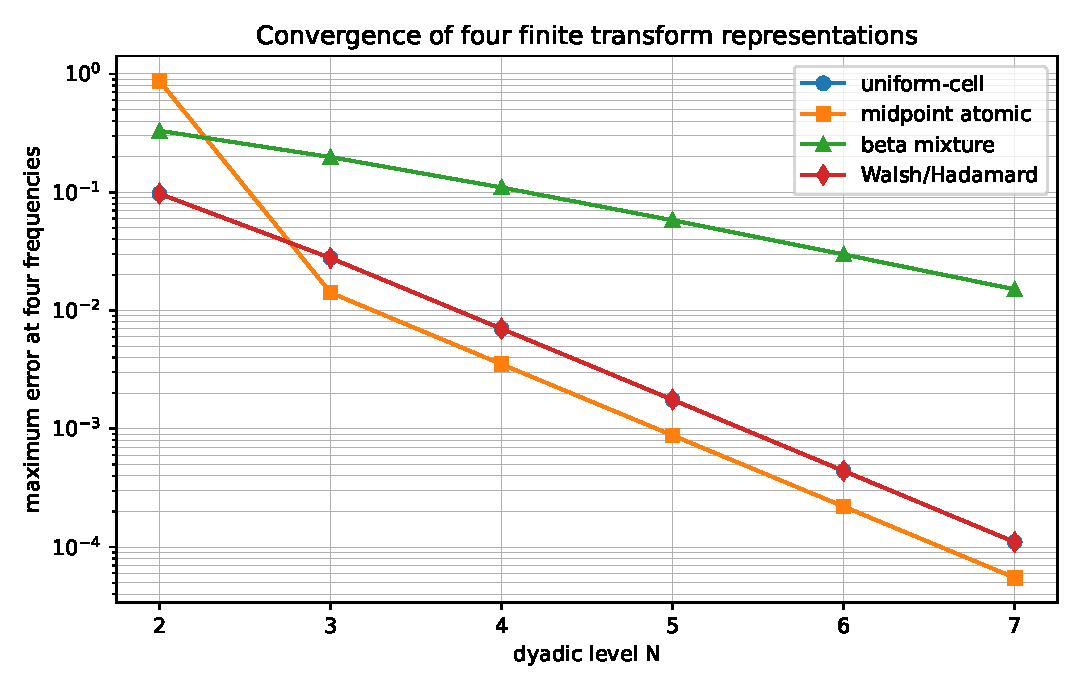
\includegraphics[width=0.84\textwidth]{multiresolution_convergence.pdf}
\caption{Convergence of the fixed-cell, midpoint-atomic, beta-mixture, and
Walsh--Hadamard transform representations at four sample frequencies.}
\label{fig:transform-convergence}
\end{figure}

\subsection{Haar energy asymptotics}

The half-integer Fourier samples give
\begin{align}
 \|p'\|_2^2&=25.8839531509750580138\ldots,\label{eq:num-p1}\\
 \|p''\|_2^2&=1656.57300166240371284\ldots,\label{eq:num-p2}\\
 \|p'''\|_2^2&=424082.688425575063737\ldots.\label{eq:num-p3}
\end{align}
The exact rational energies and the three-term approximation from
\eqref{eq:En-first-terms} behave as follows.

\begin{center}
\small
\begin{tabular}{@{}rccc@{}}
\toprule
$n$ & $E_n$ & $16\,4^nE_n$ & relative error of three terms\\
\midrule
2 & $6.2500000\,10^{-2}$ & $16.0000000000$ & $4.290\,10^{-1}$\\
3 & $2.5292927\,10^{-2}$ & $25.8999572626$ & $3.914\,10^{-2}$\\
4 & $6.2471084\,10^{-3}$ & $25.5881558642$ & $1.220\,10^{-3}$\\
5 & $1.5757619\,10^{-3}$ & $25.8172829143$ & $1.627\,10^{-5}$\\
6 & $3.9470093\,10^{-4}$ & $25.8671202723$ & $4.231\,10^{-8}$\\
7 & $9.8723379\,10^{-5}$ & $25.8797415033$ & $4.139\,10^{-11}$\\
\bottomrule
\end{tabular}
\end{center}
The scaled energy converges to $\|p'\|_2^2$, while the three-term expansion
quickly becomes much more accurate than the displayed leading convergence.

\begin{figure}[htbp]
\centering
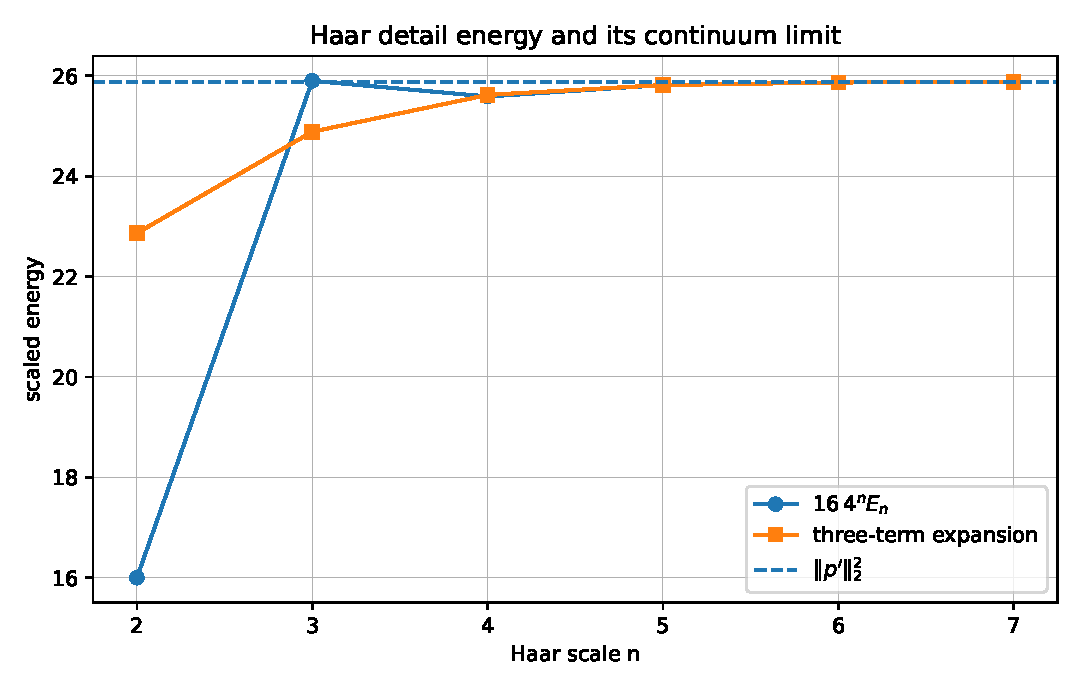
\includegraphics[width=0.84\textwidth]{haar_energy_asymptotics.pdf}
\caption{The scaled exact Haar energy, its three-term continuum expansion, and
the limiting derivative norm.}
\label{fig:haar-energy}
\end{figure}

\subsection{Reproducibility files}

The archive contains:
\begin{center}
\begin{tabular}{@{}ll@{}}
\toprule
file & purpose\\
\midrule
\texttt{numerical\_experiments.py} & fully commented exact and numerical checks\\
\texttt{numerical\_results.txt} & complete deterministic output ledger\\
\texttt{multiresolution\_convergence.pdf/.png} & transform convergence figure\\
\texttt{haar\_energy\_asymptotics.pdf/.png} & scale-energy figure\\
\bottomrule
\end{tabular}
\end{center}
The script contains independent direct and product implementations of the
Walsh transform, rather than comparing a formula with a rearrangement of
itself.

\section{Conclusions}
\label{sec:conclusions}

The central organizing object of this report is the exact dyadic mass array
$\Delta_{N,k}$.  It simultaneously yields:
\begin{enumerate}
\item a positive uniform-cell approximation and a rational exponential-polynomial
      transform limit;
\item rational unnormalized Haar coefficients and rational Faber--Schauder
      coefficients;
\item exact Walsh--Hadamard coefficients, with a finite sine--cosine product for
      every basis transform;
\item a positive beta-density mixture and a confluent-hypergeometric transform
      limit;
\item exact rational scale energies whose generating function has poles at the
      geometric lattice $4,16,64,\ldots$.
\end{enumerate}
The dual inverse array $q_{N,k}$ exchanges fixed widths and variable weights for
fixed weights and variable widths.  Its chord integrals give finite sinc
mixtures for $\Phi$ and complete homogeneous polynomial limits for the Fabius
moments.

The strongest new structural bridge is
\[
 \begin{gathered}
 \text{binary Hamming weight}
 \longleftrightarrow
 \text{Walsh vanishing moments}\\
 \longleftrightarrow
 \qbinom{N}{r}{1/2}
 \longleftrightarrow
 \text{Bell--Bernoulli higher moments}.
 \end{gathered}
\]
It complements the repository's existing $q=1/4$ moment and scale structures.
The strongest analytic bridge is
\[
 \begin{gathered}
 \text{rational Haar detail energies}
 \longleftrightarrow
 \sinc^4\text{ multiplier}\\
 \longleftrightarrow
 \|p^{(r)}\|_2^2
 \longleftrightarrow
 \text{meromorphic poles at }4^r.
 \end{gathered}
\]
Both bridges are finite and exact before limits are taken, making them good
candidates for formalization.

The most promising next steps are the two-adic classification of the coefficient
arrays, a higher-order rational multiwavelet hierarchy, phase-resolved
asymptotics of the inverse boundary coefficients, and an exact analysis of the
first Poisson aliases beyond the $\sinc^4$ energy expansion.

\appendix

\section{Compact formula index}
\label{app:formula-index}

\begin{longtable}{@{}p{0.34\textwidth}p{0.18\textwidth}p{0.38\textwidth}@{}}
\toprule
object & equation & representation type\\
\midrule
\endhead
$\Up$ & \eqref{eq:infinite-convolution} & infinite convolution of dyadic uniforms\\
$\Up$ & \eqref{eq:delta-cube} & infinite-dimensional delta integral\\
$\Up$ & \eqref{eq:BN-truncated-power} & limit of finite Thue--Morse splines\\
$\Up$ & \eqref{eq:up-head-tail} & finite spline convolved with a scaled copy\\
$\Phi$ & \eqref{eq:Phi-sinc-product} & infinite sinc product\\
$\Phi$ & \eqref{eq:qpoch-Phi} & $q$-Pochhammer product at $q=1/4$\\
$\Phi$ & \eqref{eq:zero-product} & canonical zero product with $1+v_2(n)$ multiplicity\\
$\log\Phi$ & \eqref{eq:log-Phi-zeta} & zeta power series\\
$\Up$ & \eqref{eq:up-Fourier-inversion} & Fourier cosine integral\\
$F$ & \eqref{eq:F-GilPelaez} & sine-over-frequency integral\\
$F$ & \eqref{eq:F-half-series} & half-integer cosine series\\
$p$ & \eqref{eq:p-half-series} & half-integer sine series\\
$\mathscr F_F$ & \eqref{eq:F-transform-product} & compact transform through $\Phi$\\
$\Phi$ & \eqref{eq:Phi-quantile} & inverse-Fabius quantile integral\\
$\Up$ & \eqref{eq:Legendre-Bessel} & Fourier--Legendre/Bessel coefficient integral\\
$\Up$ & \eqref{eq:Chebyshev-Bessel} & Chebyshev/Bessel coefficient integral\\
$p$ & \eqref{eq:p-Haar-limit} & rational unnormalized Haar series\\
$F$ & \eqref{eq:F-Schauder-series} & rational Faber--Schauder series\\
$\mathscr F_F$ & \eqref{eq:Fhat-Schauder} & translated $\sinc^2$ product-series\\
$p$ & \eqref{eq:p-Walsh} & rational Walsh--Hadamard series\\
$\Phi$ & \eqref{eq:Phi-Walsh-trig} & series of finite sine--cosine products\\
Walsh moments & \eqref{eq:Walsh-higher-moments} & Bell--Bernoulli finite-product coefficients\\
$F$ & \eqref{eq:F-Bernstein-limit} & limit of rational Bernstein polynomials\\
$p$ & \eqref{eq:pB-beta-density} & positive rational beta mixture\\
$\Phi$ & \eqref{eq:Phi-beta} & confluent-hypergeometric mixture limit\\
$\Phi$ & \eqref{eq:Phi-cell-limit} & fixed-width rational sinc mixture\\
$\Phi$ & \eqref{eq:Phi-quantile-chord} & equal-weight variable-width sinc mixture\\
Fabius moments & \eqref{eq:moment-cell-limit-clean} & rational fixed-cell polynomial limit\\
Fabius moments & \eqref{eq:moment-beta-limit} & rational beta-moment limit\\
Fabius moments & \eqref{eq:moment-quantile-homogeneous} & inverse-dyadic polygon limit\\
$E_n$ & \eqref{eq:En-multiplier} & $\sinc^4$ Fourier multiplier plus aliases\\
$E_n$ & \eqref{eq:En-all-orders} & Bell--Bernoulli Sobolev expansion\\
$\mathcal H$ & \eqref{eq:H-energy-generating} & meromorphic rational-energy generating series\\
$G$ & \eqref{eq:G-Schauder} & inverse Faber--Schauder series\\
$\widehat G$ & \eqref{eq:Ghat-Schauder} & inverse translated-$\sinc^2$ series\\
\bottomrule
\end{longtable}

\section{Proof details for two auxiliary identities}
\label{app:proof-details}

\subsection{Derivation of the local Haar expansion}

Let $m$ be the center of a parent interval of length $h$.  Then
\begin{align*}
 c_{n,k}
 &=h^{-1/2}\left(
   \int_{m-h/2}^{m}p(x)\dd x-
   \int_m^{m+h/2}p(x)\dd x\right)\\
 &=-h^{-1/2}\sum_{r\ge0}
   \frac{2p^{(2r+1)}(m)}{(2r+1)!}
   \frac{(h/2)^{2r+2}}{2r+2}\\
 &=-\sum_{r\ge0}
   \frac{h^{2r+3/2}}{2^{2r+1}(2r+2)!}p^{(2r+1)}(m),
\end{align*}
which is \eqref{eq:c-local-asymptotic}.  Squaring and summing midpoint samples
recovers the first coefficients in \eqref{eq:En-first-terms}; the multiplier
proof packages all integrations by parts into one $\sinc^4$ symbol.

\subsection{Absolute convergence of the first-moment Hamming layers}

Letting $N\to\infty$ in \eqref{eq:sigma-qbinom} gives
\begin{equation}\label{eq:infinite-Hamming-sigma}
 \sum_{\substack{m\ge0\\r(m)=r}}2^{-\sigma(m)}
 =\frac{2^{-r(r-1)/2}}{(1/2;1/2)_r}.
\end{equation}
Since $|a_m|\le\int_0^1p=1$, the weight-$r$ contribution formed from the first
nonzero Walsh moments is absolutely summable.  In particular, the sum rule
\eqref{eq:weight-two-sum-rule} is independent of the blockwise ordering.

\section{Reproducibility ledger}
\label{app:ledger}

\lstinputlisting[basicstyle=\ttfamily\scriptsize]{numerical_results.txt}

\begin{thebibliography}{99}

\bibitem{ProveIt}
V.~Reshetnikov,
\emph{ProveIt: Fabius Function Development}, GitHub repository,
\url{https://github.com/VladimirReshetnikov/ProveIt}, audited at commit
\nolinkurl{924652f4a9a656fd957d2936b2f053747c6f6c47}, 2026.

\bibitem{AriasDeReyna2017}
J.~Arias de Reyna,
\emph{Arithmetic of the Fabius function},
Annales de l'Institut Fourier \textbf{67} (2017), no.~2, 637--666.

\bibitem{Haar1910}
A.~Haar,
\emph{Zur Theorie der orthogonalen Funktionensysteme},
Mathematische Annalen \textbf{69} (1910), 331--371.

\bibitem{Walsh1923}
J.~L.~Walsh,
\emph{A closed set of normal orthogonal functions},
American Journal of Mathematics \textbf{45} (1923), 5--24.

\bibitem{Fine1949}
N.~J.~Fine,
\emph{On the Walsh functions},
Transactions of the American Mathematical Society \textbf{65} (1949),
372--414.

\bibitem{Schauder1928}
J.~Schauder,
\emph{Eine Eigenschaft des Haarschen Orthogonalsystems},
Mathematische Zeitschrift \textbf{28} (1928), 317--320.

\bibitem{LorentzBernstein}
G.~G.~Lorentz,
\emph{Bernstein Polynomials}, 2nd ed., Chelsea, New York, 1986.

\bibitem{Daubechies1992}
I.~Daubechies,
\emph{Ten Lectures on Wavelets},
CBMS--NSF Regional Conference Series in Applied Mathematics 61, SIAM, 1992.

\bibitem{deBoor2001}
C.~de Boor,
\emph{A Practical Guide to Splines}, revised ed.,
Applied Mathematical Sciences 27, Springer, 2001.

\bibitem{AndrewsAskeyRoy}
G.~E.~Andrews, R.~Askey, and R.~Roy,
\emph{Special Functions}, Encyclopedia of Mathematics and its Applications 71,
Cambridge University Press, 1999.

\bibitem{FrontierConfluent}
\emph{Confluent Digital Extrapolation and Lambert-Phase Tomography in the
Fabius--Rvachev System}, current research manuscript in the \repo{} documentation
corpus, 2026.

\bibitem{IntegralTransforms}
\emph{Integral Calculus and Transform Dualities for the Fabius--Rvachev
System}, current research manuscript in the \repo{} documentation corpus, 2026.

\bibitem{DyadicSpectral}
\emph{Dyadic Spectral Determinants for the Fabius--Rvachev System}, current
research manuscript in the \repo{} documentation corpus, 2026.

\end{thebibliography}

\end{document}
